\documentclass[11pt,oneside,chapters]{starlink}

\usepackage{amsfonts}
\usepackage{verbatim}
\usepackage{natbib}

\stardoccategory {Starlink Cookbook}
\stardocinitials {SC}
\stardoccopyright{Copyright \copyright\ 1999, 2001--2003, Central Laboratories for the Research Councils}
\stardocnumber   {13.1}
\stardoctitle    {Theory and Modelling Resources Cookbook}
\stardocversion  {2.5}
\stardocmanual   {\ }
\stardocabstract {
    This cookbook is intended to assemble references to
    resources likely to be of interest to theorists and modellers.
    It's not a collection of standard recipes, but instead a
    repository of brief introductions to facilities.  It includes
    references to sources of authoritative information, including
    those Starlink documents most likely to be of interest to
    theorists.

    Although the topics are chosen for their
    relevance to theoretical work, a good proportion of the
    information should be of interest to all of the astronomical
    computing community.
 }
\stardocauthors{Norman Gray}
\stardocdate{10 March 2003}

\begin{document}
\scfrontmatter

\chapter{Introduction}
\label{s:intro}

Theory work, unlike observational work, does not have a clear set
of requirements for applications programs.  There is no instrument
data to reduce, no observations to plan, and all the observational
fuss of calibration, flat-fielding, dark frames, image centroids can
be avoided.  All we need is a fast machine, and a compiler we can
trust.

Well, not quite all. This cookbook is intended to be useful at and
after the point when you start to wrestle with the computing details
of your scientific problem.  It's not a collection of standard
recipes, but instead a repository of brief introductions to facilities
you may not know existed, or didn't know how to get started on.  It
includes references to sources of authoritative information, including
those Starlink documents most likely to be of interest to theorists.
It doesn't try to teach you all of anything, but aims to give you
enough information to decide if the topic is useful, and if the
included references are worth pursuing.

Although the topics are chosen for their relevance to theoretical
work (and for the purposes of this text, I'm taking the term to
include all who develop their own modelling codes), a good proportion
of the information should be of interest to
all of the astronomical computing community.

\section{Call for contributions}
\label{s:contributions}

For such a wide ranging project, I cannot hope to have given an
ideally just account of every topic.  Please send comments,
corrections, and expansions either to me at \texttt{norman@astro.gla.ac.uk}
or to the Starlink software librarian at \texttt{starlink@jiscmail.ac.uk}.
Updates to the cookbook and its example programs can be found there.

I am particularly interested in comments on the following topics:

\begin{itemize}
\item
I'd like to include a section on Monte Carlo
simulations, but don't feel qualified to comment
myself.  Can anyone
give any pointers?

\item
The cookbook is reasonably well-stocked with
material on computation, but rather thin on more
detailed astrophysical topics (\ref{s:astro}).
It does have a section on Stellar Atmosphere models
(\ref{s:models}); what else should be here?

\item
Do I need a section on parallelization, beyond the
very brief (indeed evasive!) mention in \ref{s:optim}?
\end{itemize}

\chapter{Computing}
\label{s:computing}

Everyone should start with the
\xref{Starlink User's Guide}{sug}{}.

\section{Unix guides}
\label{s:unix}

Before you can do anything, you need to make friends with
the machine.  The slogan to remember here is `unix
\emph{is} user-friendly, it's just picky about who its
friends are'.  Keep calm, breath deeply, and make friends
with a guru.

Your first source of information might be
\xref{Starlink's Unix introduction}{sun145}{}.
This covers the basics of logging on, moving
around, issuing commands, creating files, and starting
programming.  It also includes references to other Starlink
documents which can provide more detailed help on various
aspects.

There are very good online introductions to Unix at
\url{http://unixhelp.ed.ac.uk/}
and
\url{http://star-www.maps.susx.ac.uk/help/4ltrwrd/unixman.html}.

There are numerous books on Unix.  Two which seem to be at
the right level are
``Unix Shells by Example'' \citep{quigley}
and
``Unix in a Nutshell'' \citep{nutshell}.
Both cover
the Bourne shell (\texttt{sh}) and the C shell
(\texttt{csh}), plus other utilities such as
\texttt{sed} and \texttt{awk} (see \ref{s:sedawk}).
By the way, let me put in a plug for
\texttt{bash} as a usable shell, as it includes all the
best bits of the Bourne and C shells.  The only disadvantage
of bash is that Starlink has, to some extent, standardised
on \texttt{csh}, so that setup scripts, for example, are
designed to work with \texttt{csh} alone; this is not
often a real problem, since these scripts are generally
simple enough that you can duplicate their effects `by
hand'.

You will occasionally see references to unix manual pages
followed by a number.  This indicates which section of the
manual the documentation can be found in (section 1 is
normal user commands, section 3 is standard library calls,
section 5 is file formats, and so on).  If you see a
reference to \texttt{sed(1)}, for example, you'd read
the manual page online with the command \texttt{man sed}.
A useful variant of the \texttt{man}
command is \texttt{apropos}, for example \texttt{apropos find}.
This searches the list of man-pages, and lists
all those commands which include a particular word in their
short description.


\section{Editors}
\label{s:editors}

% <update versionid="v1.1">
% <px>Expanded the description of vi</px></update>
% <update versionid="v2-0"><px>Added more vi URLs, caught
% typos</px></update></subhead>

One of the aspects of working on Unix which you'll have to deal with
pretty early in your contact with it, is which editor to use.  An
editor is the tool you use to create your documents or programs.  It's
the tool you'll use more than any other.

It's very much a personal decision, which editor you use, and when
you're feeling understimulated, you can discuss the matter with your
officemates (don't get blood on the machines, though, and remember to
wash and dry your thumbscrews carefully after use --- you'll need them
again when you discuss programming languages --- see
\ref{s:progs}).

\xref{SUN/170}{sun170}{}, ``Editors on Unix'',
is an overview of some of the available
options, listing their good and bad points.  In addition to
this, Brian McIlwrath wrote an overview of available text
editors in the September 1998 (issue 21) edition of the
\href{http://www.starlink.ac.uk/bulletin/98sep/node15.html}{Starlink Bulletin}.

Emacs is many people's favourite (and mine).  You can do
just about anything in emacs --- it's a hugely productive
environment --- but you may get cricks in your fingers from
the odd key combinations.  Emacs itself can help you up the
long learning curve: there's a very good tutorial built-in
to emacs, and available by typing \texttt{C-h C-t}
(that's control-H, control-T), plus extensive documentation
behind \texttt{C-h C-i}.  Leave emacs with \texttt{C-x C-c}
(obvious, really).

Vi is another favourite.  It is indeed very powerful, but
rather more of an acquired taste.  An advantage of vi is
that it's small, and therefore quick to start up --- this
makes it useful if you want to make a quick change to a
file, or make similar changes to a number of files, and it
makes it useful as a editor for Pine, or any other mail
program.  An even bigger advantage of vi, however, is that
it's available on every Unix system since the Ark, so if you
can use vi, you can work on whichever Unix system you find
yourself.  The main disadvantage is that it is exceedingly
unintuitive.  There's quite a lot of help available for vi
(it needs it, after all), but not, oddly enough, in the
manual page, which describes in elaborate detail how to
start up vi, but not what to do once you succeed.  You'll
find a good introduction to vi in Chapter 6 of the
``Solaris 2.6 Advanced Users' Guide'', and in
Chapter 2 of the old ``SunOS 4 Documentation
Tools'' manual, and probably in the corresponding
manual for any other Unix you use (don't worry about these
being out of date, by the way, vi doesn't change much...).
Online introductions to, and references for, vi include the
\href{http://unixhelp.ed.ac.uk/vi/ref.html}{the unixhelp manual},
\href{http://www.devshed.com/Server_Side/Administration/Vi101/Vi101/page1.html}{vi101},
and even the \href{http://www.thomer.com/thomer/vi/vi.html}{vi-lovers home page}!

If you want to leave vi without saving what you've
(accidentally?)  typed, you can do so by typing
\texttt{:q!} (if it beeps at you, or if those characters
simply appear in the typing buffer on screen, try pressing
escape once or twice first).  By the way, it's pronounced
`vee-eye', not `vye': pronounce it the wrong way and you'll
lose all your credibility (of course, if you know the
correct way to pronounce it, you'll lose all credibility
with a different set of folk --- your choice).

For VMS fans, there's \texttt{jed}, which is a simple
and fairly sane editor which includes an emulation of the
EDT editor of old.  It's available on Starlink systems, and
documented in \xref{SUN/168}{sun168}{}.

Finally, there's \texttt{pico}, the editor used
internally by the pine mailer.  You can't go wrong with this
one, but I'd imagine it could be a little painful if you're
writing much code with it.  Along the same lines, the
\texttt{textedit} editor which comes with OpenWindows
really isn't up to much.  It looks pretty, but has zero
support for programming.  You'll be using an editor \emph{a
lot}, so it's worth investing time to learn to use a
powerful one to its full extent.


\section{Numerical analysis}
\label{s:na}

Anyone writing numerical code needs \emph{some} awareness
of numerical analysis, to avoid burning up CPU time with a
hideously inappropriate and inaccurate algorithm.

By far the most accessible introduction to numerical
methods is \href{http://www.nr.com}{Numerical Recipes}
\citep{nr}, which comes in
different editions, containing code in C, Fortran and
Fortran 90.  Use the second edition: the first has a
significant number of bugs.

A large part of the book's popularity stems from the fact that its
authors are scientists rather than numerical analysts, so that they
are more concerned with producing reliable results than with a point
of view which sometimes appears to see efficiency, unshakable
robustness and algorithmic elegance as ends in themselves.  For
further discussion, and some caveats, see \ref{s.nr}.

My advice is to use ``Numerical Recipes'' for your
numerical programming until it runs out of steam on your
particular problem.  Follow the references in there, or look
at the \href{http://www.mathcom.com/corpdir/techinfo.mdir/scifaq/q165.html}{booklist}
in the on-line Numerical Analysis FAQ.  Also (perhaps
unexpectedly), I suggest you take a look at the Usenet
newsgroup \texttt{comp.lang.fortran}, even if you don't
actually use Fortran.  This is one of those happy few Usenet
newsgroups with a high signal-to-noise ratio, and listening
in on this can be profitable when the conversation turns to
general numerical analysis.  A similar resource is the
JISCmail \href{http://www.jiscmail.ac.uk/lists/COMP-FORTRAN-90.html}{comp-fortran-90}
list.

To support more specialised numerical computing, refer to the
libraries section below, \ref{s:lib}.

\subsection{Numerical Recipes}
\label{s.nr}

\href{http://www.nr.com}{Numerical Recipes}
\citep{nr} does not claim to
be a numerical analysis textbook, and it makes a point of
noting that its authors are (astro-)physicists and
engineers rather than analysts, and so share the
motivations and impatience of the book's intended
audience.  The declared premise of the NR authors is that
you will come to grief one way or the other if you use
numerical routines you do not understand.  They attempt to
give you enough mathematical detail that you understand
the routines they present, in enough depth that you can
diagnose problems when they occur, and make more
sophisticated choices about replacements when the NR
routines run out of steam.  Problems \emph{will} occur
because the routines are not written to be bullet-proof,
and if you use them thoughtlessly you can break them
without much difficulty.  Also, the routines will likely
prove inadequate if you have a very demanding application
which needs a more efficient or more specialised routine
than the ones available here.

That is, the NR library is not filled with magic bullets,
and if you try to use its contents as such, the only thing
you'll shoot is your foot.  However, NAG and SLATEC don't
supply magic bullets either (though `any sufficiently
advanced library is indistinguishable from magic to the
unsophisticated programmer', as Arthur C Clarke didn't
quite say).  You might use the NR routines successfully
for years, but if and when they fail you, you'll use the
more sophisticated substitute all the better because
you'll understand \emph{why} the simpler original was
inadequate.

It is a consequence of the book's aims that the routines
will not necessarily be the most intricately and obscurely
efficient.  Efficiency matters a lot if you are running
some huge hydro code taking months of Cray time, but I
would claim that if your code takes less than a week of
wall-time to run, then the efficiency gains from using
opaque library routines is simply not worth the cost in
debugging time.  No matter how robustly the library
routine is written, you will be able to abuse it --- you
will manage to break it somehow --- and when that happens
your only recourse is to work through pages of Fortran IV
trying to find the overflowing total, or the case you
hadn't realised was marginal.

If you need very high efficiency, then take a course on
numerical analysis and spend time understanding the
subtleties of the library routines.  Otherwise, read NR
carefully (there are sometimes important caveats in the
text), customise the routines to your problem, cross check
the results you obtain, and keep alert.  If you have an
aversion to documentation, use NAG or another library:
using the NR routines as a black box is a numerical recipe
for disaster.

Despite NR's popularity, it has its critics.  These are
typically that the NR routines do not use the most
efficient modern algorithms, and that they sometimes go
wrong in borderline situations.  While this may be true
(and will be more true of the first edition than the
second), it is largely a consequence of NR's declared
intention of being accessible and intelligible.  Without
making the point explicit, as far as I can see, the NR
authors privilege intelligibility over high efficiency,
and practicality over unabusable robustness; I don't
believe it's entirely fair, therefore, to criticise them
for not being ultra-efficient and bulletproof.  There is a
collection of criticisms of the books by W Van Snyder at
JPL, at \url{http://math.jpl.nasa.gov/nr/}, along
with some suggestions for alternatives; there is a
rebuttal from the NR authors at
\url{http://www.nr.com/bug-rebutt.html}.

From the NR home pages, you can browse and print out
chapters from the books, but you can't download the source
code.  Do remember that the NR code is copyrighted and
\emph{not} free; this may affect your ability to
redistribute code which uses it.

\subsection{Floating point representation}
\label{s:fp}

As with numerical analysis, the intricacies of how
floating-point numbers are represented, and the quirks of
their representation on different platforms, are a
maelstrom into which you can fall, dazed, confused and
unproductive.  However (and again as with numerical
analysis), if your codes become elaborate enough, then you
are going to have to take the plunge.

Even if you have no plans to venture into the deep, there
is a minimum awareness of the problems which can help you
write more robust code.

What follows here is rather detailed, but it does, I
believe, represent the majority of what you might need to
know about floating point representation; there is a good
alternative introduction in ``Numerical Recipes''
\citep{nr}, and an excellent and detailed
introduction in Chapter 2 of Sun's ``Numerical
Computation Guide'' \citep{sunncg}
(appendix E of the same book claims to be `What every
computer scientist should know about floating point
arithmetic', and is an edited reprint of
\citet{goldberg91}.  It makes interesting
reading, but it's probably more than many natural
scientists need to know).  My account here is not intended
to supplant either of these sources.  Below, I'll talk
exclusively of IEEE base-2 floating point numbers, as
defined in IEEE standard
\href{http://grouper.ieee.org/groups/754/}{IEEE-754};
there are other standards, but they're now of historical
interest only, as just about all modern machines other
than VAXes and older Crays use IEEE.  Most of what I say
concerning accuracy will be about single precision;
exactly the same issues arise with double precision, but
you can sweep them under the carpet for longer.

\subsubsection{Endianness of floating-point numbers}
\label{s:endianness}

% <update versionid="v2-4"><px>Paragraph
% transformed into section</px></update></subhead>

The IEEE standard leaves it open to chip manufacturers
to decide the order in memory of the four or eight bytes
of a floating point number (the same is true of
integers, though they're not part of the IEEE spec).
This is denoted by the endian-ness (or `bytesex') of the
machine.  Alpha and Intel chips are little-endian;
Sparcs, the Motorola 68k family used in Macs, and
Motorola PowerPC chips, are big-endian (there's also a
`PGP-endian' ordering, but that really isn't likely to
trouble anyone any more).  This generally does not
matter if you stick to a single platform (other than in
the context of programs such as those described in \ref{a:islittleendian:c}
and \ref{a:fpp:c}), but
it makes a difference if you want to share raw data
files (see \ref{ss:io}) between architectures.

% XXX Add swap-bytesex.c to distribution?

\subsubsection{Accuracy}
\label{s:accuracy}

% <update versionid="v2-0"><px>Added
%  a brief description of the format of
%  doubles</px></update>

The central insight is that \emph{you cannot represent an
infinite number of reals in a finite number of bits
without approximation}.  It is a consequence of
this that the result of any calculation will lose
precision when it is represented as a floating-point
bit pattern, and that the extent and importance of
this loss of precision \emph{depends on the
operands}.  Both of these seem obvious by
themselves, but the consequences can be sufficiently
non-obvious to trip you up.

A non-special IEEE floating-point single-precision
longword represents a number
\begin{equation}
(-1)^s \times 1.m \times 2^{e-127}
\label{e:ieee1}
\end{equation}
where $s$ (the sign),
$m$ (the mantissa or significand) and $e$ (the
exponent) are base-2 numbers represented in 1, 8 and 23
bits respectively, and $0 < e < 255$; the offset 127 is called the
\emph{bias}.  These are encoded into the 32 bits of
the longword as shown in table \ref{f:fp}.

\begin{table}
\caption{IEEE floating-point representations of numbers.
This table is adapted from table 2--3 in \citet{sunncg} and figure 1.3.1
in \citet{nr}, which have fuller discussions of the issues here.  For
discussion of $b$ and $b-1$ see the text.
\label{f:fp}}
\begin{tabular}{rlll}
                                  & $s$ & $e$             & $m$                                           \\
$1=$                              & 0   & 0 1 1 1 1 1 1 1 & 0 0 0 0 0 0 0 0 0 0 0 0 0 0 0 0 0 0 0 0 0 0 0 \\
$2=$                              & 0   & 1 0 0 0 0 0 0 0 & 0 0 0 0 0 0 0 0 0 0 0 0 0 0 0 0 0 0 0 0 0 0 0 \\
$3=$                              & 0   & 1 0 0 0 0 0 0 0 & 1 0 0 0 0 0 0 0 0 0 0 0 0 0 0 0 0 0 0 0 0 0 0 \\
$2\epsilon=$                      & 0   & 0 1 1 0 1 0 0 0 & 0 0 0 0 0 0 0 0 0 0 0 0 0 0 0 0 0 0 0 0 0 0 0 \\
$1+2\epsilon=$                    & 0   & 0 1 1 1 1 1 1 1 & 0 0 0 0 0 0 0 0 0 0 0 0 0 0 0 0 0 0 0 0 0 0 1 \\
$b = 1.000220 =$                  & 0   & 0 1 1 1 1 1 1 1 & 0 0 0 0 0 0 0 0 0 0 0 0 1 1 1 0 0 1 1 0 0 1 1 \\
$(b-1) = 2.197266\times10^{-4} =$ & 0   & 0 1 1 1 0 0 1 0 & 1 1 0 0 1 1 0 0 1 1 0 0 1 1 0 0 1 1 0 0 1 1 0 \\
\end{tabular}
\end{table}

Firstly, it is important to distinguish between the
\emph{range} and the \emph{accuracy} of
floating-point numbers.  The smallest and largest
positive numbers which can be \emph{represented} by
normal IEEE single-precision numbers are
$1.0_2\times2^{1-127}\approx1.175\times10^{-38}$
and
$1.1\dots1_2\times2^{254-127}\approx3.403\times10^{38}$,
but this is very different from the accuracy to which
these numbers are represented. These extreme values
differ from the next representable ones up and down by
$1\times2^{-23}\times2^{-126}\approx1.401\times10^{-45}$
and $1\times2^{-23}\times2^{127}\approx2.028\times10^{31}$
respectively, so that any number which differs from them
by less than that amount is unrepresentable.  This
accuracy limitation is expressed by the \emph{machine
epsilon}, $\epsilon=2^{-24}\approx5.960\times10^{-8}$
(for IEEE single-precision), which is the maximum
relative error incurred when a real number is
represented in floating-point.  It is a consequence of
this that $\epsilon$ is the
smallest number such that
$1\oplus2\epsilon\neq1$, where
the operator $\oplus$
represents addition of floating-point
numbers.
\footnote{This is a slightly different
convention from that used in, for example,
\citet{nr}, which defines
$\epsilon$ to be the smallest
number for which $1\oplus\epsilon\neq1$.}

Another way of thinking about this is as follows.  When
two floating-point numbers are added, the exponent of
the smaller one must be increased to match that of the
larger, and the mantissa (or significand),
$m$, must be shifted rightwards
to compensate.  If the two numbers differ greatly in
magnitude, then the smaller will lose significance in
this operation, and if it is less than a factor
$2\epsilon$ of the larger one,
the shift will push the number right off the end of the
mantissa, and contribute nothing to the sum.  You can
easily confirm that $2^{24}\oplus1.0=2^{24}=16777216.0$.

The immediate practical consequence of this is that if,
in the bowels of some calculation, you are adding up
many small numbers (doing an inner product for very
large vectors, for example), then the final total may be
grossly inaccurate if you've fallen into this trap.
Similarly, if you are subtracting numbers which are
almost equal, perhaps in the course of debiasing or
removing some DC offset, the subtraction may allow all
or most of the leading accurate digits to cancel,
leaving the result to be determined by digits possibly
heavily contaminated by roundoff.  [\hyperlink{ta:rw}{RW}]

Consider the simple
calculation $ab-ac$, with
$a\approx1.000244$,
$b\approx1.000220$ and
$c\approx1.000269$.  Here, the
rounding in the two multiplications conspires to give a
difference which has a huge relative error of
$2.07\times10^{-3}$.  We can,
however, address the problem by rewriting the
calculation in ways which are equivalent for real
arithmetic, but inequivalent for machine arithmetic.  If
we do the subtraction before the multiplication, and
calculate $a\otimes(b\ominus c)$,
then we retain a little precision in the
subtraction and end up with a relative error of
$9.765625\times10^{-4}$.
Finally, if we instead calculate
$a\otimes((b-1)\ominus(c-1))$,
then we do the subtraction with a full 23 bits of
precision (compare \ref{f:fp}), and lose as little
as possible of this in the final multiplication, and end
up with a relative error of only
$2.532525\times10^{-7}$.  This
is clearly a rather synthetic example, but it is not at
all unrealistic, as it is equally clearly closely
related to the common problem of calculating the
discriminant $b^2-4ac$ of the
quadratic formula, when the quadratic is nearly
degenerate.

These problems are demonstrated in
the short program \texttt{fpdemo.c} in
\ref{a:fpdemo:c}.  Note that the numbers
$a=1+1/2^{12}$,
$b=1+(1-)/2^{12}$ and
$c=1+(1+)/2^{12}$ are (a)
specifically chosen to demonstrate the effect, and (b)
are calculated within the program, rather than being
initialised from the decimal representations 1.000244,
and so on.  If the latter were not true, then the
improvement in relative error would disappear, since all
precision would have been lost in this initialisation.
If you wish to explore the representation of
floating-point numbers on your machine, you can do so
using the example program \texttt{fpp.c} in
\ref{a:fpp:c}.

These problems are unfortunately
both easy to run into, and hard to notice if you're not
in the habit of looking for them whilst writing your
code.  A brute-force way around them is to do sensitive
parts of your calculation in double precision.  If you
are doing the calculation in double precision and still
running into the problem, then you will have to
rearrange the calculation somehow, to contain the loss
of precision.
\footnote{For example, appendix E of
\citet{sunncg} displays `Kahan's summation
formula', which allows you to perform a large sum
without losing precision in the manner described
above.}
Note, however, that a compiler's
optimizer can frustrate your efforts here, if you've
given it a sufficiently high optimization level that it
starts reorganising your code: in general
$(a\oplus b)\oplus c \neq a\oplus (b\oplus c)$, and
$a\ominus b\oplus(b\ominus c)\neq a\ominus c$, but a high
optimization level may instruct the compiler to ignore
this fact, which can be disastrous for the accuracy of
your code.  Moral: make sure you know what the various
optimization levels actually do before you invoke them.

As alluded to above, it is generally possible to
sweep accuracy problems under the carpet by using
double-precision floats.  These occupy eight bytes of
storage rather than four, and the analogue of
\ref{e:ieee1} is
\begin{equation}
(-1)^s \times 1.m \times 2^{e-1023}
\end{equation}
where $s$,
$m$ and
$e$ are respectively 1, 52 and
11 bits long, and the bias is 1023.  Thus the smallest
and largest normal positive double-precision IEEE
numbers are $1.0_2\times2^{1-1023}\approx2.225\times10^{-308}$
and $1.1\dots1_2\times2^{2046-1023}\approx1.798\times10^{308}$,
and the machine epsilon for double precision is
$2^{-53}\approx1.11\times10^{-16}$.

On some platforms such as Solaris and Compaq, with the
manufacturer's compilers, it is possible to use
quadruple precision.  You should not use double or
quadruple precision automatically, however, for a
variety of practical and principled reasons.

Firstly, if your program already suffers from
rather prodigal use of memory (ie, has very large
arrays), then the doubling in the size of real arrays
will only make the problem worse and, by probably
increasing the amount of swapping, might make your
program significantly slower.

Secondly, although
there are some issues to do with the relative speed of
single- and double-precision calculations, these are
probably not significant enough to be worth worrying
about in all but the most long-running codes, and in any
case would generally be swept up by the compiler (I'd
welcome any correction or amplification on this
point).
\footnote{There used to be an issue here in that
all of K\&R C's floating-point operations were
defined to be done in double-precision --- this made
things easy for compiler writers, at the expense of
runtime.  This is no longer true in ANSI C.}

Thirdly, if your results change if you switch to
double-precision, then there is an accuracy problem in
your code, which would probably bear some investigation.
If there is some part of your code which genuinely
requires the extra precision --- say because you have to
add numbers of hugely different scale in accumulating a
large inner product --- then there is not much you can do
about it, and that part of your code, at least, must
have the extra precision.  Failing such an explanation,
however, you can regard such behaviour as a miner's
canary, indicating \emph{some} potential problem with
your code, which you might benefit from investigating
further.

Fourthly, remember that some algorithms
are designed to work with single precision, and will no
longer work properly if you search-and-replace
\texttt{double} for \texttt{float} or
\texttt{real*8} for \texttt{real*4}.  As just
one example, one of the Numerical Recipes algorithms
(\texttt{svdcmp}) includes a convergence test of,
essentially, \text{if (val+err==val)}.  Whatever
the merits or otherwise of this as a test, it is a cheap
way of establishing whether \texttt{err} has reached
machine precision, which will not work in the expected
way if \texttt{val} and \text{err} are double
precision.

For further details on floating point
representation, see, for example
\citet{hauser96}, and informal but very
useful discussions (both available on the web) by
William Kahan \citep{kahan96} and Jim
Demmel \citep{demmel}.  The former is one
of the authors of the IEEE-754 standard for
floating-point numbers.

\subsubsection{Other floating-point topics}
\label{s:otherfloat}
% <update versionid="v2-1"><px>Added table of compilers
% and enabled IEEE traps</px></update>
% <update versionid="v2-2"><px>Mention that x.ne.x is true
% when x is a NaN</px></update>

As well as defining the format in which normal floating-point numbers are
stored, the IEEE-754 standard includes the definitions for several
other (classes of) special values.

When the exponent $e$ (of a single-precision number) is zero,
the longword is taken to represent the number
\begin{equation}
(-1)^s \times 0.m \times 2^{-126}
\label{e:ieeedenorm}
\end{equation}
(compare \ref{e:ieee1}.
Unlike the usual floating-point numbers, which have an implied leading
1 in the significand and 23 bits of precision, and which are referred
to as `normalised', these have an implied leading 0 and less than 23
bits of precision.  These are `denormal' or `subnormal' numbers, and
are the result of an underflow, such as dividing the smallest
normalised number by two.  This behaviour is known as `gradual
underflow', and allows the precision in a calculation to degrade
gracefully when it underflows.  It is distinct from `Store-0
underflow' common before the IEEE standard, in which any expression
which underflowed was replaced by zero.  This was, and remains, one of
the more contentious parts of the IEEE standard.  Be warned that older
Crays, which use their own floating-point format, have a Store-0
underflow policy, and that the Alpha chip, although it generally
implements IEEE floats, has a Store-0 underflow as its default mode,
and will neither produce, nor accept as input, denormalised numbers.

If the significand as well as the exponent is zero, the longword
represents the number $(-1)^s \times 0$.  Note that the IEEE zero
is \emph{signed}, which allows $1/(+0)$ and $1/(-0)$ to be
positive and negative infinity; this can be important when doing
calculations near branch points.

If the exponent is 255 and the significand is zero, the longword
represents the value $(-1)^s \times \infty$.  That is, infinity has a
special value, distinct from the largest possible normalised number.
Positive infinity is generated by, for example $1/0$, or $\log 0$,
where infinity is the mathematically correct, but otherwise
unrepresentable, value of a calculation.

If the exponent is 255 and the significand is non-zero, the
longword is \emph{Not a Number}, usually represented by the string
`NaN'.  A NaN is the result of an operation on invalid operands, such
as $0/0$ or $\log(-1)$.  NaNs have the properties that any
operation which has a NaN as an operand has a NaN as its result; and
any comparison on a NaN, such as \texttt{<} or \texttt{==},
evaluates to False, including \texttt{NaN==NaN}.  The only exception
is that, when \texttt{x} is a NaN, then \texttt{x != x} is
true.  Why would you
want to use such a peculiar number?  Generally you don't, and its
appearance in a calculation is an error, which is why processors can
be set to dump core when a NaN or an Infinity is produced.  However,
it can be useful to turn off this behaviour if it is not off by
default, and rather than elaborately avoid producing a NaN at each
stage, make a check once at the end of a calculation, possibly
invoking an alternative (possibly more expensive or special-cased)
algorithm if any NaNs are found.

Different compilers handle exceptional values in different
ways; see \ref{t:traptab}.  Of the three Starlink platforms,
only the Alpha traps on exceptional values by
default.

\begin{table}
\caption{
Summary of compiler IEEE traps.
\label{t:traptab}
}
\begin{tabular}{llll}
Compiler      & traps enabled by default                    & see                                 & suppress with \\
Sun cc \& f77 & none                                        & \texttt{-ftrap}                     & \\
Alpha cc      & overflow, divide-by-zero, invalid operation & -fptm, -ieee                        & -ieee \\
Alpha f77     & overflow, divide-by-zero, invalid operation & -fpe                                & -fpe1 \\
gcc           & none                                        & \texttt{-mfp-trap-mode} (Alpha-gcc) & \\
\end{tabular}
\end{table}

We have only scratched the surface of a rather
intricate topic here.  Both Suns and Alphas have
extensive \texttt{f77} and \texttt{cc}
man-pages, which hint at the broad range of
floating-point options available when compiling and
linking your code.  See \ref{s:optimnan} for
discussion of the efficiency tradeoffs when using IEEE
exceptional values.


\section{Programming languages}
\label{s:progs}

% <update versionid="v2-0"><px>Mention of SUN/209 in the
% context of dynamic memory allocation in Fortran.</px></update>

\begin{quotation}
I speak Spanish to God, Italian to women, French to
men, and German to my horse.
\emph{Emperor Charles V} (attr.)
\end{quotation}

There is no One True Programming Language, nor even One True
Compromise.

The language you use to write code is as much a function of your
background, environment and personal tastes, as it is a function of
technical merit.  At some level or another, all programming languages
are equivalent, but just as you'd look askance at anyone who wrote a
stellar atmosphere code in TeX
\footnote{Not impossible.  Since
someone has already done the hard work of implementing a
BASIC interpreter in TeX (honestly!), you'd simply have to
port your code to BASIC and let it rip.},
it's clear that
some languages are more suited for some tasks than others.

The obvious issue at this point is the choice between
Fortran and C.  Let me state first of all that, \emph{for
general scientific computing}, I do not believe the
difference between the two is substantial enough, or the
advantages of each are unqualified enough, that it warrants
abandoning the language you're comfortable with and learning
the other.

The languages' respective strengths only become significant
when you are deep within their `native territories': for
Fortran this territory is that of numerically intensive
codes with week-long runtimes, for C it is intricate
manipulation of data structures.  Away from these extremes,
the choice is at the level of which to choose for a
particular application, given that you know both, and an
ideal application might be said to be one with a Fortran
heart whirring away in a C harness.

Though Fortran and C are both simple languages, Fortran is
simple in ways that an optimizing compiler can exploit.
This means that for a numerically intensive application,
where processing speed is very important, Fortran is the
only suitable language.

Why is this?  The reason can be illustrated by the two
languages' loop semantics.  Fortran's loop is very simple:

\begin{terminalv}
   do 10, i=1,n
C  process array element a(i)
10 continue
\end{terminalv}

The equivalent construction in C is

\begin{terminalv}
    for (i=0; i<n; i++) {
       /* process array element a[i] */
    }
\end{terminalv}

The difference is what the two language compilers can say about the
loop. The Fortran compiler can know that the loop
will be performed exactly $n$
times, since neither \texttt{i} nor \texttt{n} may be changed within the loop; also the array \texttt{a(i)}
cannot overlap with any other array within the loop body.  On the
other hand, in C, the loop
\texttt{for (init; test; increment) { body }} is defined to be
equivalent to
the loop \texttt{init; while (test) {
body; increment; }}, so that both \texttt{i} and
\texttt{n} could change within the loop, and since \texttt{a}
could be a
pointer, it could point \emph{anywhere}.  The Fortran
compiler could
rewrite the first loop as

\begin{terminalv}
      do 10, i=1,n,4
C     process array element a(i)
C     process array element a(i+1)
C     process array element a(i+2)
C     process array element a(i+3)
   10 continue
\end{terminalv}

cutting the number end-of-loop tests by a factor of four (this is a
simple example of `loop unrolling', and presumes that
$n$ is divisible by 4).  The loop
semantics could also make the elements of the loop
candidates for parallelization, if the compiler and hardware support
that
\footnote{Note that, with pipelining, RISC chips can typically
support some degree of on-chip parallelization, even for a single
CPU.}
The C compiler has to do a lot more investigative work before
it can make any similar rearrangements.

Even if there were no such fundamental differences, the fact would
remain that Fortran vendors have always sold their products on the
strength of their optimizers, so that it is both easier \emph{and}
profitable for Fortran compilers to produce very fast code.

Though C's loop semantics are troublesome, it is really the pointer
type which causes a lot of the trouble --- since a pointer is little
more than an address, the compiler can have little clue what the
programmer is aiming to do with it, and so has little choice but to
make a literal translation of the C code into assembler.

The pointer type is redeemed, however, because it is this which
allows C to code complicated data structures so naturally: not only
aggregate types, but linked lists, queues, and all the other ways of
holding, reading, parsing and generally juggling data, so beloved of
Computer Science 1.

Fortran 90/95 goes some way towards addressing Fortran's
weaknesses by introducing pointers (though the fact that
they're living in a Fortran code doesn't make them any less
troublesome to an optimizer), as well as proper data
structures and some modularisation.  At the same time as
Fortran does that, however, C++ uses object-orientation to
further enhance C's advantages in data manipulation, going
so far as to make functions auxiliary features of data
structures.

For general discussions of the issues involved in high-performance
computing, see the book
``High Performance Computing'' \citep{dowd}.

Starlink ensures that C, C++, Fortran 77 and Fortran 90/95 compilers
are available at all sites.

\subsection{Fortran 77}
\label{s:fortran77}
% <update versionid="v1.1"><px>Added
% pointers to Fortran standard
% document.</px></update>

Fortran 77 is probably the dominant current Fortran dialect,
replacing earlier standards such as Fortran IV and Fortran 66\footnote{A
statement like that can't be made without some qualification.
Depending how you added it up, you could probably make a case that old
Fortran dialects probably have more code actually running on CPUs,
since many heavily-used libraries were written a long time
ago.}.  There are several dialects of Fortran, containing
various vendors' language extensions, but the only extensions which
are usually portable are those in VAX Fortran, which includes the
\texttt{enddo} statement for terminating do-loops, and the
\texttt{\%val()} function which is necessary to intermix Fortran
and C code (see \ref{s:candf}).

The \href{http://www.fortran.com/fortran/F77\_std/rjcnf.html}{standards document for Fortran 77}
is not exactly bedtime reading,
but can be quite useful when you have forgotten details of syntax,
especially to make sure what you are writing is correct rather than
just allowed by the compiler you are using at the time.  As an
introduction to Fortarn 77, I've heard good things about
\citet{metcalf85}. [\hyperlink{ta:mbt}{MBT}]

An important deficiency in Fortran is its lack of any
standard way of dynamically allocating memory (as opposed
to allocating arrays to be a fixed size at compile time).
The Starlink CNF library,
\xref{SUN/209}{sun209}{pointers} is intended to make
this reasonably easy, and includes a brief discussion of
the underlying mechanism.  This is rather a can of worms,
but the essential technique is to write a bit of C which
obtains a pointer to a block of memory via a call
\texttt{malloc}, return that pointer to the Fortran
program as an integer, then use \texttt{\%VAL()} to
supply that integer as an argument to a function which is
expecting an array.  This is non-standard (and not likely
to become standard, now that Fortran 90 includes its own
mechanisms for dynamic memory allocation), but it is a
well-established technique and therefore probably more
portable than you have any right to expect.

% Dynamic memory allocation in Fortran:
% How about a section on hacking dynamic memory allocation in Fortran 77,
% since it's the one thing that you really can't do if you stick to the
% standard?  I don't know whether it makes sense to go into detail, but it
% could be useful to mention what the options are, e.g. vaxisms
% (or other non- standard constructs) and where you can expect
% them to be supported, using Starlink CNF, writing your own fortran
% wrapper for malloc, DIY allocation from a statically allocated
% common block.  On the other hand it's a bit of a can of worms,
% perhaps it's getting a bit specific for a document like this. (MBT)

There is a large number of introductions to Fortran, but not, I
believe, a single preeminent one.  The
``Starlink application programming standard'',
\xref{SGP/16}{sgp16}{},
is a collection of programming style guidelines for Fortran,
and includes further references.

There is a reasonable amount of online information on
Fortran, which is well-covered at the `Fortran Market'
(\url{http://www.fortran.com/fortran/info.html}),
which includes several Fortran FAQs.


\subsection{Fortran 90/95}
\label{s:fortran90}

Almost immediately after Fortran77 was standardised, work began on
its successor.  Although this project was named Fortran 8X, the work
took long enough that the final standard was named Fortran 90.

The Fortran standard is maintained by ISO committee
\href{http://www.nag.co.uk/sc22wg5/}{JTC1/SC22/WG5},
and the current version of the standard is
\href{http://www.nag.co.uk/sc22wg5/IS1539-1\_1997.html}{ISO/IEC 1539-1 : 1997}.

Fortran 90 was an attempt to respond to the numerous developments in
language design, seen since Fortran's last standardisation in the
sixties and seventies.  In contrast to Fortran 77, which aimed to
standardise existing practice, Fortran 90 was an attempt to push
forward the development of Fortran as a language.  A summary of the
new features (adapted from \citet{metcalf96}) is:

\begin{itemize}
\item
Free format source code form (no more column-counting).

\item
A means for the language to evolve by labelling some features as
`obsolescent'.

\item
Array operations (for example,
\texttt{X(1:N)=R(1:N)*COS(A(1:N))}).

\item
Pointers.

\item
Improved facilities for numerical computation
including a set of numeric enquiry
functions.

\item
User-defined derived data types composed of arbitrary data
structures and operations upon those
structures.

\item
Facilities for defining collections called
`modules', useful for global data definitions and
for procedure libraries.  These support a safe
method of encapsulating derived data types.
Operator overloading and prototyping.

\item
Requirements on a compiler to detect the use of
constructs that do not conform to the syntax of the
language or are obsolescent.

\item
New control constructs such as the \texttt{select case} construct,
an \texttt{exit} and a
new form of the \texttt{do}.

\item
The ability to write internal prodedures and
recursive procedures, and to call procedures with
optional and keyword arguments.

\item
Dynamic storage (automatic arrays, allocatable
arrays, and pointers).

\item
Improvements to the input-output facilities,
including handling partial records and a
standardized \texttt{namelist}
facility.

\item
Many new intrinsic procedures, (date, precision,
arrays, ...)
\end{itemize}

Fortran 90 is backwards compatible with Fortran 77, so
that every \emph{strictly} conformant Fortran 77 program
is also a valid Fortran 90 program.  However, many of
Fortran 77's odder features are strongly deprecated, and
may disappear in the next revision of Fortran, due to
appear sometime in the next decade.  Fortran 95 is a minor
revision of Fortran 90.

There is an increasing number of books on Fortran 90/95;
for a booklist, refer to the Fortran Market at the URL
above.  I am, of course, reluctant to recommend books I
have not used myself, so I will simply note that I have
heard good things about \citet{metcalf96},
and that the first author was prominent in the
negotiations concerning the development of the Fortran 90
standard.

If you plan to use Fortran 90/95, but avoid the
deprecated parts of Fortran 77 altogether, you might be
interested in \href{http://www.swcp.com/~walt/imagine1/}{F},
which is a subset of Fortran 90 with all the deprecated
features removed.  You can obtain an F compiler from
Imagine1, including a free educational version for
Linux.

Several Fortran compilers were reviewed in a short
\href{http://www.liv.ac.uk/HPC/FortranCompilerStudyHTML/FortranCompilerStudyHTML.html}{report}
of January 1997 by the high performance computing project
at Liverpool.

It is occasionally necessary to produce code in a mixture
of Fortran and C.  See \ref{s:candf}.

\subsection{C}
\label{s:c}

There are hundreds of books on C, but the only
\emph{essential} one is the Kernighan and Ritchie book
\citep{kr} (also known as just `K\&R').
This is a very short book, by the authors of the language,
which combines a tutorial introduction with a detailed
reference to the language and its standard libraries.  I
believe it's the only C book you'll ever need.

The book's compression makes it possible, and even
advisable, to read it from beginning to end.  It avoids
the bloat found in many other C books by not teaching you
how to program, by never saying anything twice, and by
never attempting the empty reassurance that `it's all
easy, really'; its examples often illustrate more than one
point at a time, and culminate in a sample implementation
of the library function \texttt{malloc}.  Science
textbooks don't talk down to you; I don't see why computer
texts should be excused for doing so.

It follows from this that K\&R is not necessarily the
ideal recommendation for someone new to programming, who
might need something a little more comprehensive.  My
recommendation in that case is to find an introductory C
(or even general programming) book which covers what you
want without irritating you, and use that up to the point
where you feel comfortable with K\&R.

C allows the programmer a considerable degree of freedom
in how an algorithm is expressed.  The fact that this
freedom is easily abused makes style guides more common
for C than for other languages.  Starlink has adopted
``The Elements of C Programming Style'' by Jay
Renade and Alan Nash as its principal C programming
standard, as well as producing a compact collection of
programming style suggestions in \xref{SGP/4}{sgp4}{}.

One way of making your life easier in this respect is to
be consistent about using current standard ANSI-C.  See
\ref{s:compilers}.

The C language as originally designed by Kernighan and
Ritchie was standardised as ANSI-C in 1990 (K\&R 2nd
edition describes the latter).  This standard is currently
being revised by an ISO working group with the memorable name
\href{http://std.dkuug.dk/JTC1/SC22/WG14/}{ISO/IEC JTC1/SC22/WG14 --- C}.
One of the motivations to
the work is to provide better support for floating point
calculations in C, such as defining a standard interface
to the IEEE floating point exceptions.

The excellent
\href{http://www.eskimo.com/\%7Escs/C-faq/top.html}{C FAQ}
contains \emph{substantially} more than you
realised you wanted to know about C.  It contains detailed
discussions of both common and arcane problems.


\subsection{C++ and object orientation}

C++ is an object-oriented version of C, and was finally
standardised in 1997.  Compiler makers have tracked the developing
standards, so that recent C++ compilers should conform pretty
closely to the standard even if they formally pre-date it.

Object-orientation is the notion that functions are
\emph{attached to} data, rather than simply operating on
them.  For example, if a C program were to declare a data
type \texttt{Array}, and initialise a variable of that
type with \texttt{Array a;} then one can imagine a
function to return the determinant of the array, declared
as \texttt{float determinant (Array a);}.  In C++, the
`function' to obtain the determinant could be declared as
\emph{part of the data type}, and obtained via the
expression \texttt{a.determinant()}.  There are two
main points to this.  Firstly, the so-called `member
function' \texttt{determinant} can have privileged
access to the internal representation of the data type
\texttt{Array}, so that other parts of the program
need not, and may not, manipulate that representation,
erroneously or otherwise.  Secondly, and consequently, the
representation and matching member functions can be
\emph{changed} with the guarantee that the rest of the
program will be unable to tell the difference.  This is
characterised in the remark that new programs have always
been able to use old code (in libraries), but
object-oriented approaches mean that old programs can use
new code (when an implementation changes, while the
interface remains the same).

Of course, both of these points are to some extent true
of traditional programming languages --- indeed I'd doubt
that there's anything you can do in C++ which you couldn't
do with some ingenuity in C --- but the point is that they
are much easier, and much more natural, in C++.

It may be clear at this point that C++ is not a
beginner's language.  The result of grafting a high-level
abstraction onto portable assembler is a language with far
more syntax than is healthy.  Do not feel you need to
learn C before C++ --- they are closely enough related that
the differences can be confusing.  My feeling, however, is
that you should consider learning Java (\ref{s:java}) first if you have the time: there is
relatively little that needs to be unlearned going from
Java to C++, and Java's simplicity makes it easier to come
to grips with object-orientation, without drowning in a
sea of punctuation.

The excellent
\href{http://www.parashift.com/c++-faq-lite/}{C++ FAQ}
includes book recommendations.  The canonical
book for C++, with the same status K\&R has for C, is
``The C++ Programming Language''
\citep{stroustrup}, by the language's author.
However, I find Stroustrup's book rather irritating: it's
rather badly organised, and the index is
\emph{dreadful}.

Note, by the way, that the C++ compiler on Suns is named
\texttt{CC}, on Alphas named \texttt{cxx}, and on
Linux named both \texttt{c++} and
\texttt{g++}.


\subsection{Java}
\label{s:java}

% <update versionid="v1.1"><px>Added a description of Java's model of
% compiling to interpreted bytecodes, to the extent that this relates to
% efficiency and speed.</px></update>
% <update versionid="v2-0"><px>Pointed out that JITs make Java a candidate for high-end codes,
% pointing to the Java Grande Forum for
% details.</px></update>
% <update versionid="v2-3"><px>Hoisted the Java section up a level, and added some remarks about
% efficiency and profiling.</px></update>

Java was developed by Sun and at present (mid-2002)
eclipsed only by XML as the current Big Thing.  Source
code is compiled to machine-independent bytecode, which is
then either interpreted, or compiled to machine code on
the fly, by a Java Virtual Machine (JVM) on a particular
platform.  The main interest to astronomy might be in
developing machine- and architecture-independent
interfaces either to codes or archives.  It's also, I
think, of use as a stepping-stone to C++, since its
object-oriented features are less obscured by syntax than
they are in C++.  A very good textbook, written (you won't
be surprised to guess) by two of the language's authors,
is 
``The Java Programming Language'' \citep{arnold98};
once you've mastered the
basics, there's a good deal of helpful advice in
``Effective Java'' \citep{bloch01}.
There are numerous resources at Sun's Java site at
\url{http://java.sun.com}.

Java is a mixture of an interpreted and a compiled
language.  Java source code is compiled by the Java
compiler into bytecodes, which are then interpreted by a
Java Virtual Machine.  These bytecodes are low-level, but
architecture-independent so that, in principle, only the
virtual machine and its runtime need to be ported to a new
machine, whereas the code should be completely portable.
This does not work quite as well in practice as it does in
principle, but it does mean that Java is not too far off
the ideal of run-anywhere code.

Since Java bytecodes are ultimately interpreted, Java
programs have the potential to be rather inefficient.
However, just-in-time compilers (JIT), which analyse
running code and optimize the most heavily-used parts, and
similar developments, should help the situation improve in
the future.  This is possible because JITs have access to
both the program source code and the running program, and
so can combine the features of both an optimizer and a
profiler, and thus optimize more aggressively than a
traditional compiler could.  This, combined with Java's
good built-in support for different platforms and for
resource-discovery, means that, possibly somewhat
surprisingly, Java has been suggested as a suitable
language for high-end codes.  The
\href{http://www.javagrande.org/}{Java Grande Forum}
is concerned with investigating and
promoting developments in this area.

Note that it is relatively easy to write slow Java (for
example, adding Strings is a \emph{lot} slower than
using a StringBuffer; input and output streams are not
(extensively) buffered, so if you have a lot of I/O, you
would be well advised to use
\texttt{Buffered{Input,Output}Stream} objects wrapping
your I/O objects; small-object creation is extensively and
increasingly optimised, but it's still not dirt-cheap, so
look out for that in a small loop).  That means that using
a profiler (see \ref{s:profiling}) is particularly
important.  However, with Java, that's easy, because
there's one built in to the JVM.  Give the option
\texttt{-Xrunhprof:help} to find out how to invoke it.
For example: 

\begin{terminalv}
java -Xrunhprof:cpu=samples,file=myprog.hprof myclass
\end{terminalv}

There's quite a lot of information in
here (and the file format is under development), but as
with all profilers, you'll see a list of the number of
times various methods were called: the ones at the top of
the list are the ones where the program spent most of its
time, so work out why, and concentrate on making them
faster.  Ignore the rest.

Java is still developing.  At present (mid-2002) Java
1.3.1 is long in the tooth but stable.  Version 1.4 is in
beta, and on the point of being released properly; it
includes a few changes to the language, most noticeably
the inclusion of an \texttt{assert} construct.


\subsection{Other languages}
\label{s:otherlang}

C and Fortran cover most of the bases for scientific computing, but
there are one or two others which come in useful occasionally.

\subsubsection{awk and sed}
\label{s:sedawk}

Often, you can find yourself performing some repetitive
editing task, for example massaging data into a form
which a program can conveniently read.  Such tasks can
conveniently, and reliably, be done by programs such as
\texttt{awk} and \texttt{sed}.  Neither of these
utilities is as well-known as it should be, as they can
save a great deal of tedious and error-prone effort.

\texttt{sed} is a version of the \emph{very}
simple editor \texttt{ed}, which is specialised for
performing edits on a stream of text.  For example, the
following rather elaborate \texttt{sed} script
prints all the section headings from a LaTeX document:

\begin{terminalv}
sed -n 's/^\\\(sub\)*section{\(.*\)}.*\$/\2/p' sc13.tex
\end{terminalv}

This may look like
gibberish, but it is simpler than it looks.  The option
\texttt{-n} instructs \texttt{sed} not to print
out input lines, which it does by default.  The
\texttt{sed} expression in quotes calls the
\texttt{s} command: whenever the `regular
expression' between the first pair of slashes matches,
the \texttt{s} command replaces it with the
expression between the second pair and, because the
\texttt{s} command is suffixed with a
\texttt{p}, prints out the modified line.  The
regular expression matches lines which start with a
backslash, have zero or more occurrences of the string
`sub', which is followed by the string
`\texttt{section{}', then any sequence of
characters, followed by a \texttt{}} then any
characters, ending at the end of the line.  The caret
\texttt{\^} matches the beginning of a line, the
backslash is a special character, so that it must be
`escaped' by prefixing it with another backslash,
\texttt{\textbackslash\textbackslash}, the grouping operators are
\texttt{\textbackslash{}(} and \texttt{\textbackslash{})}, the asterisk
indicates that the previous (bracketed) expression may
be present zero or more times, the dot matches any
character, and the dollar matches the end of the line.
As well as grouping, the parentheses save what they
match, and the expression \texttt{\textbackslash{}2} in the
replacement text refers to what the second pair of
parentheses matched, namely the text between the curly
braces.  The overall result is that the matched string
(the whole of the line) is replaced by the contents of
the braces and then, because of the \texttt{p}
suffix, printed.

Another useful tool is \texttt{awk}, named after
its designers Aho, Weinberger and Kernighan.  Like
\texttt{sed}, it works through a text file,
executing scraps of code whenever a line matches some
condition.  Before it does anything with a line, it
breaks it into fields, separated by whitespace by
default.  Consider the following example\footnote{There
are two versions of \texttt{ps} on Suns --- this
example assumes you are using the
\texttt{/usr/ucb/ps} version.}

\begin{terminalv}
ps u | sed 1d | \
   awk '{print $4, $0; totmem+=$4}; END {printf "total memory: %f\n", totmem}'
\end{terminalv}

This (not terribly useful) line generates a process
listing using \texttt{ps}, uses \texttt{sed} to
delete the first line (that is, it executes the command
\texttt{d} on line number 1), and then passes the
result through the \texttt{awk} program contained in
quotes.  On every line, this prints field number 4 (the
\texttt{\%MEM} column in the listing) and field 0
(which is \texttt{awk}-speak for the whole input
line), and adds the value of the fourth field to a
running total; on the line matching the pattern
\texttt{END} --- that is, the pseudo-line at the end
of the file --- \texttt{awk} prints out the
accumulated total.

You won't typically generate expressions as complicated
as these on the fly (at least, not until you get
\emph{really} good).  This example is intended to
suggest that you can, in aliases or in scripts, perform
quite complicated transformations of text files.  For
further details you could look at the \texttt{sed}
or \texttt{awk} man-pages, which are complete but
very compressed, or work through a tutorial in your
system's printed documentation.  There are several
guides to \texttt{sed} and \texttt{awk}, but you
might be best off, initially, using an advanced
introduction to Unix, such as
\citet{quigley} or
\citet{nutshell}.  The canonical
documentation for regular expressions is on the
\texttt{ed(1)} manual page.

\subsubsection{Perl}

% <update
% versionid="v1.1"><px>Added pointer to the Schwartz
% reference, and a description of Perl's
% compile-then-interpret model.</px></update>

Perl is a general-purpose scripting language.  It
started off as a text-reformatting facility, rather like
a super-\texttt{awk}, but it has now grown to the
point where it really is a programming language in its
own right, capable of supporting quite substantial
projects.  Perl programmers can call on a huge range of
supporting code, collected at the Comprehensive Perl
Archive Network, \href{http://www.cpan.org}{CPAN},
to do everything from internet programming to database access.
Perl's expressive power makes it ideal for rapid
development of all sorts of complex systems --- some huge
proportion of the web's CGI scripts, for example, are
written in Perl.  Unfortunately, the flexibility of
Perl's syntax make it quite possible to write spaghetti,
the like of which we have not seen since Fortran IV
dropped out of fashion.

The Perl manual pages
are reasonably clear.  O'Reilly publishes a good book on
Perl, written by Larry Wall, its author
\citep{wall}.  This is a good reference
book, but \citet{schwartz97} is possibly a
better tutorial introduction.  Perl regular expressions
are \emph{slightly} different from the ones used by
\texttt{sed} and friends --- see the
\texttt{perlre} manual page.

Perl is a
semi-interpreted language.  Somewhat like Java, when the
Perl interpreter first processes your Perl script, it
compiles it to an internal code, which it then proceeds
to interpret.  This means that Perl programs have a
relatively long startup time, but run reasonably
efficiently after that.  This is not a big issue in most
applications.

The current (end-2001) version of
Perl is 5.6 or thereabouts.  Perl 6 will be a
significant step in the evolution of the language: it's
in the offing, but still some way away.


\section{Code topics}
\label{s:codetopics}

Several of the topics mentioned here are discussed at greater length
in the Sun Fortran User's Guide \citep{sunf77}, which is of interest
even if you program only in C.

\subsection{Profiling}
\label{s:profiling}

Before you start doing any optimization at all, check which parts of
your code are slowing the machine down --- there's no point in
tweaking, for example, a one-time initialisation routine which takes
only a tiny fraction of the program's runtime.  You do this by using a
profiler.

Different compilers will invoke a profiler (presuming
they have one) in different ways.  The Sun and Digital
Fortran compilers include profiling code if you give the
option \texttt{-pg} to the \texttt{f77} command.
Compile \emph{and} link the program with this option (if
you wish, you can compile only those modules you want to
profile with the \texttt{-pg} option, but you must
include the option in the final link command), and then
run it.  This run will create a file \texttt{gmon.out}
in your current directory.  Then you can run
\texttt{gprof}.  Taking as example the programs in
\ref{a:profiling}, we can build and profile them as
follows:

\begin{terminalv}
% f77 -pg -o timewaster p1.f p2.f p3.f
p1.f:
MAIN silly:
p2.f:
mkidentity:
p3.f:
determinant:
Linking:
% timewaster
1.00000
% ls
gmon.out        p1.o            p2.o            p3.o
p1.f            p2.f            p3.f            timewaster*
% gprof timewaster > timewaster.gprof
\end{terminalv}

The output file \texttt{timewaster.gprof} is many lines long, even
though the program is so short!  The file contains a great deal of
information, but buried amongst it is the following display (from the
Sun profiler, trimmed):

\begin{terminalv}
called/total       parents
index  %time    self descendents  called+self    name    	index
called/total       children

0.05        0.64       1/1           main [2]
[1]     97.2    0.05        0.64       1         MAIN_ [1]
0.64        0.00  100000/100000      mkidentity_ [4]
0.00        0.00       1/1           __s_wsle_nv [167]
0.00        0.00       1/1           determinant_ [8]
0.00        0.00       1/1           __do_l_out [157]
0.00        0.00       1/1           __e_wsle [158]
 -----------------------------------------------
0.64        0.00  100000/100000      MAIN_ [1]
4]     90.1    0.64        0.00  100000         mkidentity_ [4]
\end{terminalv}

This indicates that the subroutine \texttt{mkidentity}
was called 100000 times from the main program, and that
90.1\% of the time --- a total of 0.64 seconds --- was spent
in that routine.  Were this a real project, this would
indicate that this routine would be a good one to examine
for speedups.

This example, and a further one using the
\texttt{tcov} utility, were taken from
\citet{sunf77}, which might be consulted for
further details.  \texttt{pixie} is the corresponding
utility on Compaqs --- see its man-page for details
[\hyperlink{ta:rw}{RW}].

\texttt{gprof} is not specific to Sun, but is
available for other architectures, and other compilers
(including \texttt{gcc}) as well.


\subsection{Optimization}
\label{s:optim}

Just say no!  Or, if you need authority:

\begin{quotation}
\emph{Donald Knuth, in ``Literate Programming''}

Premature optimization is the root of all evil.
\end{quotation}

The first thing to ask yourself, when you are considering
performance enhancements on your code is `do I really need
to do this?'.  You should only attempt optimizations once
you have either identified a particular part of your code
which needs improving, or else you \emph{know} that you
can write the efficient version of the code correctly.  If
the `efficient' version is unnatural, then the savings in
runtime you achieve by reordering the code have a good
chance of being wiped out by the time spent debugging a
convoluted juggling act.  Within reason, prefer simplicity
and robustness to efficiency\footnote{However, there is
\emph{no} excuse for Bubble Sort!} --- get
your code working correctly and believably, and only then
start worrying about speed.  That way, if you later
establish that you need to work on part of the code, you
at least have a trusted set of results to check the new
version's against.  Another way of putting this is that
it's easier to optimize correct code than it is to correct
optimized code.

If you're writing a code which will run for days or more,
then it might be worthwhile investing a significant effort
in tuning your code for performance.  Doing this properly
might involve you learning more about your machine's
architecture than you might enjoy, and as as result will
make your program less portable to the next generation of
whizz-bang hardware, or even the next compiler.

It is generally worthwhile to use hand-optimized
routines, if they are available for your compiler.  Where
this can pay particularly good dividends is in the case of
linear algebra, where the speed of a calculation can be
significantly improved (`a factor of several') by routines
carefully written to access memory in an optimal way.
There is a standard interface to such routines called the
BLAS (Basic Linear Algebra Subroutines), which your
compiler documentation may mention.
% XXX : find info
% about BLAS from the Sun and Alpha compiler docs, and check
% these Netlib URLs.  Mention LAPACK?
Although it won't
be as fast as a machine-specific implementation, the free
\href{http://www.netlib.org/blas/}{BLAS implementation at Netlib}
(\href{http://sunsite.doc.ic.ac.uk/packages/netlib/blas/index.html}{UK mirror})
should speed your codes up
significantly. [\hyperlink{ta:mbt}{MBT}, \hyperlink{ta:rw}{RW}]

The first lesson to learn about optimization is that the
compiler can probably do it better than you can.

Most compilers will have a \texttt{-On} option, to
allow you to set how aggressive the compiler's
optimization will be.  The GNU gcc compiler, for example,
allows optimization levels 1, 2 and 3, and Solaris Fortran
has five levels, which progressively enable more
techniques for improving your program's execution speed.
Compaq compilers have a `\texttt{-tune host}' option,
to produce code optimized for a particular machine.
[\hyperlink{ta:mbt}{MBT}]

If your program starts behaving oddly, at some point you
should start worrying about errant optimization, if you
have that turned on.  Optimization works by the compiler
recognising patterns in your code, and possibly
rearranging the output assembly language to take advantage
of these.  If it gets this wrong (because there's a bug),
if your program relies on a particular floating-point
behaviour, or if you're doing something sufficiently weird
with your programming language that you manage to confuse
the compiler, then you could trick it into doing the wrong
thing.

Specifically, if you have occasion to worry about the
order in which expressions are evaluated --- for example to
conserve precision, as described in \ref{s:accuracy}
--- then you should be very wary of optimization, as one of
the first things an optimizer \emph{might} do is to
reorder expressions which are associative mathematically
but not computationally.  If you have some code like this,
it might be best to isolate a single routine in a module
of its own and compile it separately with its own
appropriate optimization level.

Parallelization is another type of optimization.  Just
say no several times to this, but if you have an
application which really needs it, then buy a book and
some aspirins.  See \ref{s:ncbooks}.

Although you should generally leave optimization to the
compiler, there are some things you can do to at least
avoid getting in its way.

\subsubsection{Avoid using the \texttt{register} keyword in C}

% <update versionid="v1.1"><px>Rewritten following
% comments</px></update>

This is, historically, supposed to suggest to a
compiler that a particular variable might be better
stored in a register than in main memory, though the
actual semantics defined in the C standard is that the
keyword is an assertion that the program nowhere takes
the address of the variable so qualified.  Such an
assertion means, amongst other things, that the variable
will never be visible from any other functions, which
might trigger other optimizations.
[\hyperlink{ta:sg}{SG}]

You do not need to use this keyword to actually suggest
to the compiler that it store the variable in a
register, since the compiler might well do this anyway,
and have a better idea of which (non-obvious, or
temporary) variables to choose than you have.
% XXX : discuss this with Sergio

\subsubsection{Walk through arrays in the correct order}
\label{s:arrays}

% <update versionid="v1.1"><px>Updated/corrected comments
% on page faults by adding MBT's comments on cache
% faults.</px></update>

A multi-dimensional array is necessarily stored in
memory as a linear array.  If you have to process this
entire array, it will be fastest if you try to do so in
the order in which the array is stored.  Fortran arrays
are stored with the leftmost index varying fastest.
That is, the Fortran array \texttt{integer i(2,2)}
will be stored in memory in the order
\texttt{i(1,1)}, 
\texttt{i(2,1)},
\texttt{i(1,2)} and
\texttt{i(2,2)}

Take,
for example the Fortran array \texttt{integer ia(1000,1000)}.
If you run through this array
with the first index changing fastest, as in the
following fragment

\begin{terminalv}
      do 10, j=1,1000
        do 20, i=1,1000
          call some_calc (ia(i,j))
   20   continue
   10 continue
\end{terminalv}

then
you will move through the array in the `natural' order.
If, however, you process it in the other order, with the
second index changing fastest, then when you move from
\texttt{ia(i,j)} to \texttt{ia(i,j+1)}, the
computer will have to jump 1000 places forward in the
stored array, each time round the loop.  This would not
matter \emph{too} much if the entire array were stored
in physical memory, but this will not be the case for
any sizable matrix, so that to find the appropriate
array element, the machine may have to reload part of
its memory from a saved version on disk.  Such input is
relatively slow, and if the calculation is laid out in
such a way that this happens repeatedly in an inner
loop, which is executed many times by an outer loop,
then there can be a significant impact on your program's
performance.

This system of swapping memory back
and forth to disk is known as `virtual memory', and the
machine's discovery that the memory it needs is swapped
out is known as a `page fault', and is one of the
important statistics about the run of your program.  You
can obtain such statistics in copious detail by using
the compiler's profiler (see \ref{s:profiling}),
or quickly by using the \texttt{time} command (see
your system's \texttt{time} man-page for details ---
not all versions provide this information by default).

Of course, it's not really as simple as just
that.  Even when the entire array \emph{is} stored in
physical memory, or when you have rearranged your
program to minimise the number of page faults, it can be
important not to hop about in arrays too much.  Modern
architectures will typically have a small amount (modern
PCs around half a Mb, biggish servers around 8 Mb) of
memory called `cache' which has much faster access time
(typically an order of magnitude or more) than the bulk
of the RAM.  The relationship between this and core RAM
is strongly analogous to the relationship between core
RAM and disk, in that cache-lines (which are like memory
pages, but typically only a few words long) get swapped
in and out of it when one word from the line is
required.  The upshot of that is that it's important to
avoid hopping about over distances much smaller than an
I/O page since, even if you have no page faults, cache
faults make a huge difference.  And of course it's not
as simple as that either --- sometimes there are two
levels of cache, some architectures implement some sort
of prefetching, and so on.  Except with some rather
sophisticated profilers (which generally have to be
supported by a processor architecture which keeps a
record of these things) it's not really possible to see
how many cache faults you're getting, except by writing
the code more efficiently and seeing what the difference
is.  [\hyperlink{ta:mbt}{MBT}]

Unlike Fortran,
C arrays are stored with the \emph{rightmost} index
increasing fastest, so that the array \texttt{int i[2][2]} will be stored as
\texttt{i[0][0]},
\texttt{i[0][1]},
\texttt{i[1][0]} and
\texttt{i[1][1]}.

\subsubsection{I/O}
\label{ss:io}

% <update versionid="v1.1"><px>Added
% remarks and examples on raw IO</px></update>
% <update versionid="v2-0"><px>Checked
% fwrite/fread syntax, and discussed unformatted IO in
% Fortran.</px></update>

Input and output are slow, and the faster processors become, the
bigger is the cost of I/O relative to CPU cycles.  That means you
should think twice before writing out intermediate results, for reuse
later in the same calculation or another.  For example, it's quite
easy to fall into the trap of `saving time' by reading in a
precalculated table of values, without realising that it can take more
time to read the file than it would take to recalculate the table from
scratch each time.  Remember that computers don't get bored, and don't
mind doing the same calculation repeatedly.

If you do need to save values for later use, and don't
mind doing it only semi-portably, you can save time and
precision by using raw I/O rather than formatted ASCII
[\hyperlink{ta:rw}{RW}].
A C example is:

\begin{terminalv}
FILE *ofile; float arr[10];

/* set arr[i] to have sensible values */

ofile = fopen ("output-c.dat", "w");
fwrite ((void*)arr, sizeof(arr[0]), 10, ofile);
fclose (ofile);
\end{terminalv}

Note that we carefully cast the variable
\texttt{arr} to type \texttt{void*}, and that we
could replace this by \texttt{(void*)\&arr[0]} if
we thought it was clearer.  Note also the minor trick of
using \texttt{sizeof(arr[0])} rather than the more
obvious \texttt{sizeof(float)}; they are equivalent,
but the first will remain correct even if we change our
mind about the size of the elements of the array
\texttt{arr}.  You would read the contents of this
file in using the function \texttt{fread}.

The \texttt{fwrite} and \texttt{fread}
functions are not portable in general, since they deal
with floating point numbers merely as bundles of bits,
and pays no attention to how these are interpreted.
This means that such files are not portable between
machines which interpret these bits differently, so that
files written on a little-endian machine (see \ref{s:fp})
will be gibberish if read on a big-endian
machine, and vice-versa.  However, C's raw I/O is
\emph{semi}-portable, inasmuch as the
\texttt{fwrite} function above does nothing other
than copy $10\times4$ bytes
(in this case) from memory to disk; \texttt{fread}
similarly copies bytes from disk to memory without any
interpretation.

The corresponding Fortran example is

\begin{terminalv}
      real arr(10)

C     set arr() to have sensible values
      open (unit=99,file='output-f.dat',form='unformatted')
      write (99) arr
      close (99)
\end{terminalv}

Note that Fortran unformatted output is not portable in
any way.  Unlike C raw I/O, the Fortran compiler is free
to store the information on disk in any way it likes,
and the resulting file will not, in general, have
$10\times4$ bytes in it.  That
is Fortran unformatted I/O is machine- \emph{and compiler-}specific,
and the file
\texttt{output-f.dat} in this example will only be
readable in general using a Fortran program built using
the same compiler.


\subsubsection{Use NaN and Infinity}
\label{s:optimnan}

% <update versionid="v1.1"><px>Mention
% speed tradeoffs, following
% comments</px></update></subhead>

As described in \ref{s:otherfloat}, any operation
which has a \texttt{NaN} as input, produces a
\texttt{NaN} as its result.  Similarly, the special
values positive and negative \texttt{Infinity} are
legitimate numbers which can appear in a calculation.
Consider the following code fragment:

\begin{terminalv}
      do 10, i=-5000,5000
         do 20, j=-5000,5000
            if (j .ne. 0) then
               t(i,j) = real(i)/real(j)
            else
               t(i,j) = 0.0
            endif
   20    continue
   10 continue
\end{terminalv}

The \texttt{if} test is to avoid a division-by-zero
error.  If this loop were buried deep within a hierarchy
of other loops, then the test could be the source of a
significant fraction of the runtime.  It can, however be
omitted, allowing the matrix \texttt{t(i,j)} to
include numerous \texttt{Infinity}s and one
\texttt{NaN} (due to 0/0).  Because both of these
values are permissable floating-point operands, they can
be allowed to percolate through the rest of the
calculation without elaborate further tests, to be
checked only at the end.  This is possible only if the
floating-point environment is set up \emph{not} to
generate signals on floating-point exceptions (see also
\ref{s:otherfloat}).

Note that calculations involving the exceptional values
tend to run more slowly than those using normal values,
so if your calculation produces a significant number of
exceptional values --- like the artificial example above
--- a switch to IEEE semantics might not produce a speed
win overall.  Note also that the expression
\texttt{(a.lt.b)} is \emph{not} equivalent to
\texttt{.not.(a.gt.b)}, since both
\texttt{a.lt.b} and
\texttt{a.gt.b} are false
when one of the variables is an IEEE exceptional value:
this could produce hard-to-find bugs if you were not
alert to this when you were writing the code.
[\hyperlink{ta:sg}{SG}]


\subsubsection{Remove debugging options}

It may or may not be obvious that debugging and
profiling options, as discussed in \ref{s:debugging} and \ref{s:profiling},
will both slow your program down (especially in the latter
case), and make it bigger.  You should compile your
program, or at least the numerically intensive parts of
it, without them when you are not debugging it. 
[\hyperlink{ta:mbt}{MBT}]


\subsubsection{Choose a fast compiler}

Random points:

\begin{itemize}
\item
This is a case where free software is not
necessarily better.  Both Sun and Compaq expend
resources on making their compilers as efficient
as possible.  If speed is important to your
application, you're probably best off using one of
these compilers.

\item
On the Alpha, it's worth while using the
Fortran 90 compiler even for Fortran 77 code
[\hyperlink{ta:sg}{SG}].
\end{itemize}

\subsubsection{Further reading}
\label{s:ncbooks}

Take a look at the Sun Numerical Computation Guide
\citep{sunncg}, particularly the end of
chapter 5, and at the collection of papers at
\url{http://sunsite.doc.ic.ac.uk/sun/Papers/SunPerfOv+references/},
particularly the helpful paper about compiler switches:
\texttt{you\_and\_your\_compiler} (this is a generally
useful collection of Sun papers, by the way).

If you \emph{do} need to spend significant effort
tuning your code, then you should consult a textbook on
the matter.  A good one is
``High Performance Computing'' \citep{dowd}.  This
reference touches on parallelizing your code, a topic
which I have deemed sufficiently arcane not to be
discussed at all in this introductory guide.

\subsection{Debugging}
\label{s:debugging}

One approach to debugging is the brute-force method:
simply scatter tracing statements through your code and
watch them fill your screen.  There are some types of
debugging for which this is ideal --- for example, graphing
a trace of intermediate values may reveal that an
algorithm is showing signs of instability --- but it can be
very cumbersome.

Better, in many cases, is to use a debugger.  A debugger
allows you to roam through your code, stopping in
troublesome functions, examining data, and stepping
through your code line-by-line.  There is a great deal you
can do with a debugger, but they are not often the easiest
tools to master.  However, there is a good deal you can do
armed only with experience of the foothills of the
debugger's learning curve.

I will describe the Sun debugger \texttt{dbx}, here.
The use of the GNU debugger, \texttt{gdb}, and the
\texttt{dbx} debugger on Digital Unix, are broadly
similar.

First, compile \texttt{crash.c}, listed in \ref{a:crash:c},
in the usual way (\texttt{cc -o crash crash.c}),
run it, and watch it crash when it tries
to dereference a zero pointer.  This leaves a
\texttt{core} file in the current
directory\footnote{If you don't get a core file, it might
be that you have your shell set to prevent it --- possibly
as a (reasonable) precaution to avoid filling up filespace
with `useless' core files.  The command \texttt{ulimit -c}
(\texttt{sh}-type shells only) will show the
maximum size of core file: setting this to zero inhibits
creating core files, and setting it to a very large number
or to \texttt{unlimited} allows core files to be
created.  On \texttt{csh}-type shells, the
corresponding command is \texttt{limit coredumpsize unlimited}}.  You can obtain rudimentary
post-mortem information from this core file with
\texttt{dbx}, as follows:

\begin{terminalv}
% dbx crash core
[...]
program terminated by signal SEGV (no mapping at the fault address)
(dbx) where
=>[1] bananas(0x0, 0x1, 0xef691338, 0x10074, 0x2, 0xeffff8d0), at 0x10870
[2] main(0x1, 0xeffff94c, 0xeffff954, 0x20800, 0x1, 0x0), at 0x108fc
(dbx) quit
\end{terminalv}

The \texttt{where} command to \texttt{dbx} shows
where the program was when it crashed (the
\texttt{[...]} shows where I have omitted some
unenlightening chatter from the debugger).

The other information \texttt{dbx} gives you is less
useful --- the debugger doesn't know enough about your
program to be more helpful.  You can, however, tell the
compiler to pass on more information to the debugger when
it processes your code; do this with the \texttt{-g}
flag to the compiler, as in \texttt{cc -g -o crash crash.c}.
If you compile several modules to produce
your executable, you'll need to give this option to the
compilation of each module you wish to debug.  You'll also
have to give this option at the link stage on SunOS4, but
not on Solaris or for \texttt{gdb} on Linux.

If we run \texttt{crash} again now, and look at the core file, we see
that the debugger can provide us with more information.

\begin{terminalv}
% dbx crash core
[...]
program terminated by signal SEGV (no mapping at the fault address)
Current function is bananas
12           printf ("banana split: %d\n", *zp);
(dbx) where
=>[1] bananas(i = 0), line 12 in "crash.c"
[2] main(), line 22 in "crash.c"
(dbx) print i
i = 0
(dbx) print buf
buf = "banana number 0
"
(dbx) print *zp
dbx: reference through nil pointer
(dbx) print zp
zp = (nil)
(dbx) quit
\end{terminalv}

Note that we can examine the values of variables in scope
at the point where execution stopped, and that
\texttt{dbx} knows enough about C (or Fortran) to know
the type of variables it is asked to print.  Printing the
value of the pointer \texttt{zp} shows us why our
program has crashed.

The debugger is not only useful for such post-mortem
diagnosis.  It is also (for some people, primarily) used
for investigating a program's behaviour when it is running
normally, albeit with bugs we wish to track down.  For
example, start the debugger and tell it to stop when it
enters the function \texttt{bananas}:

\begin{terminalv}
% dbx crash
[...]
(dbx) stop in bananas
(2) stop in bananas
\end{terminalv}

You can set multiple breakpoints (so called) not only in functions,
but also at line numbers, or linenumbers within files (using
\texttt{(dbx) stop at crash.c:12}).  Then tell the
program to start running:

\begin{terminalv}
(dbx) run
Running: crash
(process id 29707)
Entering the bananas function: 1
stopped in bananas at line 6 in file "crash.c"
6       sprintf (buf, "banana number %d\n", i);
(dbx) next
stopped in bananas at line 7 in file "crash.c"
7       if (i != 0)
(dbx) print i
i = 1
\end{terminalv}

Note that, as well as output from the debugger itself, we
also see output from the running program.  If the program
required input from the user, it would receive it as
normal.  The program stops at the first line of code
within the \texttt{bananas} function.  We can move one
line forward in the code, verify that the parameter
\texttt{i} has its expected value, then tell the
program to resume execution.

\begin{terminalv}
(dbx) cont
banana number 1
No bananas left!
stopped in bananas at line 6 in file "crash.c"
6       sprintf (buf, "banana number %d\n", i);
(dbx) print i
i = 0
(dbx) cont
signal SEGV (no mapping at the fault address) in bananas
at line 12 in file "crash.c"
12           printf ("banana split: %d\n", *zp);
(dbx) quit
\end{terminalv}

The Solaris debugger can be used through a GUI: give the
command \texttt{debugger} to start this up.  The Digital
GUI debugger is \texttt{ladebug}.  There is a GUI
interface to \texttt{gdb}, called \texttt{xxgdb}.

In general, you can't debug optimized code (that is, code
compiled with the option \texttt{-O}), because the
optimizer may rearrange lines or remove redundant
variables.  However, both \texttt{dbx} and
\texttt{gdb} do have support for debugging code with
mild optimization, though there are some things, such as
stepping from line to line, you might not be able to do.

This introduction has merely scratched the surface of
what you can do with the debugger, by showing you the bare
minimum of commands you need to navigate around your
running program.  There is a great deal more information
available in Sun's debugging manual
\citep{sundebug}, or in \texttt{gdb}'s
info pages (\texttt{info gdb}).

\subsection{Intermixing Fortran and C}
\label{s:candf}

Because there are so many reliable subroutine libraries
written in Fortran, you will sometimes need to call a
Fortran routine from C.  Likewise, you might need to call
a low-level C routine from a Fortran program.

For a detailed overview of such `mixed language
programming', see \xref{SUN/209}{sun209}{},
``CNF and F77 Mixed Language Programming'', which
gives a detailed introduction to calling each language
from the other, as well as a set of C macros to help
support this.  I will not duplicate the contents of that
guide, but instead give a very compressed introduction to
the problem.  This might be enough to get you going.
There is a further discussion of the issues, and a
compressed description of the solutions, at the Cambridge
High Performance Computing Facility (HPCF), at
\url{http://www.hpcf.cam.ac.uk/mixed.html}.  For a
Sun-specific discussion, see Chapter 12 of
\citet{sunf77}.

The biggest difference between C and Fortran is that `C
is call-by-value, Fortran is call-by-reference'.  What
that means is that when a C function is called, it
receives the \emph{values} of its arguments, so that any
changes to them disappear when the function finishes, but
when a Fortran function is called, it receives a
\emph{reference to} its arguments, so they can be
altered easily within the function.  The consequence of
this is that when you call a Fortran function from C, you
should pass arguments using C's address-of
operator,\texttt{\&}, and when you call a C
function from Fortran, you will typically need to pass it
the \emph{value} of the variable using the
\texttt{\%val()} function (this is a non-standard VAX
Fortran extension, but one which is now so ubiquitous that
it's safe to use).  These remarks apply to unstructured
types such as characters, integers and floats --- arrays
and strings present other problems, as described below.
It follows from what I've said that if a C function is
declared as \texttt{void subr (int *p)}, it's
expecting (the value of) a pointer to an integer, so that
this could be called in the `normal' way from fortran:
\texttt{call subr (ia)}, where \texttt{ia} is an
integer variable.

See \ref{a:mixed} for example programs.

\subsubsection{Arrays}

Fortran's arrays are simple: an array of any dimension
is just a list of locations in memory, stored in the
order \texttt{a(1,1)}, \texttt{a(2,1)}, and so
on (see \ref{s:arrays}); when a Fortran function
is given an array argument, what it actually receives is
a pointer to the `top-left' element.  If you're calling
Fortran from C, you simply have to be aware of the
switch on order, and then pass
\texttt{\&a[0][0]}.

If you have a C routine with a one-dimensional array
argument (either \texttt{void func (int a[])} or
\texttt{void func (int *a)}), and you want to call
it from Fortran, you can call it simply by giving the
array name as an argument: \texttt{call func (a)}.

Passing a multi-dimensional array \emph{to} a C
function is potentially problematic.  However, you'll
almost never need to do that, because Fortran very
rarely needs to invoke C to do a numerical calculation.
If the C declaration is \texttt{func (int a[][3])},
for example (that is, an array of three-element arrays),
then a Fortran array \texttt{integer a(3,}$n$\texttt{)} could be
passed simply, as \texttt{call func (a)}.  If, on
the other hand, the C declaration were \texttt{func (int **a)}
(that is, a pointer to pointer to integer,
with the actual array elements separately allocated),
then the above Fortran array could \emph{not} be
passed as shown (and no, smarty, \texttt{call func (\%loc(a))}
wouldn't work, even though it's the
right type).  If you \emph{do} need to call such a C
function, you'll probably have to provide a suitable C
wrapper for it, and call that from the Fortran code.
C's array/pointer syntax is elegant, but not ideally
suited for numerical work\footnote{A little known
factoid for C enthusiasts: did you know that C's array
reference syntax is commutative, since \texttt{a[i]}
is defined to be equivalent to \texttt{*(a+i)} and
is thus equal to \texttt{i[a]}?  This means that
\texttt{a[3]} is the fourth element of the array
\texttt{a}, and so is \texttt{3[a]}!  Bizarrely
enough, the latter is a legitimate array reference, but
one you're probably best not including in your own
code.}.

\subsubsection{Strings}

C strings are simple objects: they are by definition
arrays of characters, with the end of the string marked
by a zero byte.  The internal structure of Fortran
strings is not defined, so that they could be stored in
whichever way is most convenient to the author of the
compiler; typically, however, they are an array of
characters with a length encoded with them.  The
practical upshot of this is that you simply cannot pass
strings back and forth between Fortran and C code in a
\emph{portable} way, and it is fortunate that you
rarely need to do this.  On those occasions when you do
need such a facility, you can use a library of
conversion routines such as those described in
\xref{SUN/209}{sun209}{}.


\subsubsection{Compiling and linking}
\label{s:compilingcf}

When a Fortran compiler produces object code,it
\emph{typically} adds an underscore to the end of each
function name.  That is, the subroutine:

\begin{terminalv}
      subroutine func1 (i)
      integer i
      call func2 (i)
      end
\end{terminalv}

will produce object code with an external symbol
\texttt{func1\_} calling a subroutine named
\texttt{func2\_}.  You must be aware of this when you
compile Fortran code which is to be linked with C
functions.  There are two ways of dealing with this.

First, you can call this subroutine from C by calling
it with the correct name:

\begin{terminalv}
int i1;
extern void func1_ (int *i);
/* call it */
func1_ (&i1);
\end{terminalv}

So far so good.  The problem arises when you want to
call C from the Fortran function, since the Fortran
function will expect to link against a function with a
trailing underscore.  If the C function is written by
you, then you could provide this, but if it is a library
routine, you will have to tell the compiler not to add
the underscore to the external name when it generates
object code.  For Sun's \texttt{f77} compiler, you
do this with the compiler option
\texttt{-ext\_names=plain}, for the GNU
\texttt{g77} compiler it is with the
\texttt{-fno-underscoring} option, and for
\texttt{f77} on the Alpha, it is \texttt{-assume nounderscore}
[\hyperlink{ta:rw}{RW}].  Note
that this will apply to all function names in that
module.  Sun's compiler also allows you to declare that
a function is in a C module, using a pragma, but this is
obviously non-portable, and so is not recommended.  On
this subject, [\hyperlink{ta:rw}{RW}] points out that
to get access to main() via f77 on decs, you need to set
\texttt{-nofor\_main} at link time.

You should, in general, use the Fortran compiler to
link the object files into an executable.  This calls
the linker with all the correct Fortran libraries.  It
is of course possible to do the same with the C
compiler, but requires a much more elaborate call.


\subsection{Compilers, and other stray remarks on code}
\label{s:compilers}

% <update versionid="v2-0"><px>Advice to use prototypes, to
% avoid another class of silly errors; added all-warnings
% switches for Sun and
% Compaq.</px></update>

Using Fortran's \texttt{implicit none} keyword is a
Good Idea.  The tiny amount of typing time you save by
relying on Fortran's automatic declaration of variables,
is more than likely wiped out by the debugging time spent
clearing up silly problems \texttt{implicit none}
would have avoided from the beginning.

Similarly, in C, use ANSI-C rather than older `K\&R'
C, and use prototypes religiously.  That is, if you have a
module \texttt{myfuncs.c}, then create a header file
\texttt{myfuncs.h} containing the prototypes of the
functions within it, and include it (\texttt{\#include "myfuncs.h"})
both in any modules which use those
functions and inside \texttt{myfuncs.c} as well.  That
way, if you change the interface to any functions in that
module, the compiler will prompt you to change the calls
to that function \emph{everywhere} that it is used.
This way, the compiler can help you avoid a whole class of
embarrassingly silly problems.

Make your code portable.  Unless you are specifically
targetting your code at a particular (supercomputer)
processor, or magic parallelizing compiler, you will save
yourself time in the long run by not making assumptions
about the machine or compiler environment.  Especially
given the imminent arrival of 64-bit machines, you are
probably not doing yourself any favours by, for example,
assuming that integers are four bytes.  Probably more
pertinently, exploiting compiler-specific features might
prevent you running your code on some new faster
architecture.  If you do decide to use some non-portable
features, you can make the future porting effort easier by
having second or third thoughts about precisely how to use
them, and by isolating them into a few subroutines, rather
than scattering them throughout your code.  It follows
that....

Compiler Warnings Are Your Friend.  Try compiling your
codes with compiler warnings switched on (with the option
\texttt{-Wall} on GNU compilers, \texttt{+w2} on
Sun Workshop compilers, and \texttt{-w0} on Compaqs).
You might be surprised at the number of peculiarities and
non-standard features this exposes, each of which is a
potential portability problem for the future.  Don't treat
compiler warnings as irrelvant nagging --- each of them is,
to some extent, an error you have made, which has the
possibility of turning round and biting you later.  I
would particularly advise this if you develop using GNU
compilers, as these seem particularly liberal about
standards: \texttt{gcc} in particular seems happy to
take any old nonsense, say `I know what you mean', and
produce code from it --- in my experience it usually
guesses my intentions correctly, but I don't want to rely
on it.  You can also adjust the strictness of the C
compiler's conformance to the ANSI-C standard by using
compiler options (Sun: \texttt{-Xa} and
\texttt{-Xc}; DEC: \texttt{-std1}; GNU:
\texttt{-ansi} and \texttt{-pedantic}).  Having
said all this, I don't want to overstate the importance of
compiler warnings: the main plank of this advice is to
spend time now to save time and aggravation later, but
this tradeoff is unlikely to be in your favour if you
spend time removing every last anomaly from your code.


\section{Link farms}
\label{s:linkfarms}

At the end of each section of this cookbook, I'll include a
collection of web-based resources you can use to search for
further information.  These will typically be either FAQs
(lists of `frequently asked questions') or `link farms'
(thematic collections of links with little further
detail).

\subsection{Unix documentation and standards}

\begin{itemize}
\item
\href{http://www.pasc.org/abstracts/posix.htm}{POSIX}
is the term for a suite of applications program
interface standards to provide for the portability of source code
applications where operating systems services are required. POSIX is
based on the UNIX (Registered trademark administrated by the Open
Group) Operating System, and is the basis for the Single UNIX
Specification from The Open Group.
[IEEE PASC (Portable Application Standards Committee)]

\item
This is currently (2001-06-20) undergoing revision by the
\href{http://www.opengroup.org/austin}{Austin Group}

\item
The POSIX standard is

\begin{enumerate}
\item
``IEEE Std 1003.1 Standard for Information technology --- Portable
Operating Systems Interface (POSIX) --- Part 1: System Interface [C
language binding]'', which is identical to ``ISO/IEC JTC1 IS 9945-1
Standard for Information technology --- Portable Operating Systems
Interface (POSIX) --- Part 1: System Interface [C language binding]''

\item
``IEEE Std 1003.2 Standard for Information technology --- Portable
Operating Systems Interface (POSIX) --- Part 2: Shell \& Utilities'',
which is identical to ``ISO/IEC JTC1 IS 9945-2 Standard for
Information technology --- Portable Operating Systems Interface (POSIX)
--- Part 2: Shell \& Utilities''.
\end{enumerate}

...and these cost money
(\href{http://standards.ieee.org/catalog/olis/licenses/licenses.html}{lots})
to buy on paper.

\item
\href{http://www.opengroup.org/onlinepubs/007908799/}{Single Unix specification},
from the Open Group
(\href{http://www.opengroup.org/publications/catalog/web.htm}{other publications}).
My understanding from the PASC document above is
that Single Unix is broader than POSIX, and covers more of the
environment (bit vague, here).  It feeds into the POSIX/ISO
standardisation process, but is not a formal standard itself.  Single
Unix does, however, have the great advantage of being available
online.

\item
The link with
\href{http://www.UNIX-systems.org/}{The Unix System} is, I fear,
rather obscure to me, but it appears that
the latter is the public face of the Open Group's
labours.

\url{http://www.geek-girl.com/unix.html}: The `Unix
Reference Desk'.  This is a very useful collection of
pointers to unix documentation.

% Disappeared
% <p><url>http://www.softlab.ece.ntua.gr/unix/docs/</url>:  This is a Greek
% collection of documents (some of which are otherwise difficult to track
% down) in a mixture of text and postscript.

\url{http://www.faqs.org/faqs/unix-faq/faq/}:
the General Unix FAQ, full of arcana.  This is one of several FAQs
which cover Unix and related issues; for some others, look at
\url{http://www.faqs.org/faqs/by-newsgroup/comp/comp.unix.questions.html}

\url{http://uk.yahoo.com/Computers_and_Internet/Software/Text_Editors/vi/}:
Collection of links to vi documentation at Yahoo.
\end{itemize}

\chapter{Theory support}
\label{s:theory}

\section{Computer algebra}
\label{s:maple}

Starlink provides access to computer algebra by supporting
the Maple package.  You might have access to Maple on your
own Starlink node, but if not, you may use it on the machine
\texttt{star.rl.ac.uk}, if you have an account there.
If you are a Starlink user, you should apply for an account
by mailing \texttt{star@star.rl.ac.uk}.

Maple allows you to enter mathematical expressions using a
fairly natural syntax, substitute into them, simplify them,
differentiate and (with limits) integrate them, and finally
go on to graph them.  As an added bonus, you can also
produce output in C, Fortran and LaTeX.

For example, consider the following example.

\begin{terminalv}
star:nxg> maple
    |\^/|     Maple V Release 4 (Rutherford Appleton Laboratory)
._|\|   |/|_. Copyright (c) 1981-1996 by Waterloo Maple Inc. All rights
 \  MAPLE  /  reserved. Maple and Maple V are registered trademarks of
 <____ ____>  Waterloo Maple Inc.
      |       Type ? for help.
> gi := amp * exp(-(xparam^2/sa^2)/2);
                                                   2
                                             xparam
                         gi := amp exp(- 1/2 -------)
                                                 2
                                               sa
\end{terminalv}

We start up Maple, and enter an expression for a gaussian.
Maple makes an attempt to display the result intelligibly.
If we had ended the expression with a colon rather than a
semicolon, Maple would have suppressed the display.  Note
that undefined variables represent themselves, and that
Maple knows that \texttt{exp} is the exponential
function, so that it knows, for example, how to
differentiate it.

Now define the variable \texttt{xparam}, and redisplay
\texttt{gi}.

\begin{terminalv}
> xparam:= cos(theta)*(xc-x0);
      xparam := cos(theta) (xc - x0)

> gi;
                                             2          2
                                   cos(theta)  (xc - x0)
                     amp exp(- 1/2 ----------------------)
                                              2
                                            sa
\end{terminalv}

Then differentiate the gaussian, and assign the result to
\texttt{gid}.  The result is something you're happy not
to have had to work out yourself.

\begin{terminalv}
> gid := diff (gi, theta);
                                                                 2          2
                                2                      cos(theta)  (xc - x0)
        amp cos(theta) (xc - x0)  sin(theta) exp(- 1/2 ----------------------)
                                                                  2
                                                                sa
 gid := ----------------------------------------------------------------------
                                           2
                                         sa
\end{terminalv}

If that the purpose of this was to do a calculation
somewhere, you might want to code this expression in
Fortran.  Doing this by hand would be error-prone, but Maple
can produce output in Fortran as well as this
`prettyprinted' style.

\begin{terminalv}
> fortran (gid,optimized);
      t1 = cos(theta)
      t4 = (xc-x0)**2
      t6 = sa**2
      t7 = 1/t6
      t10 = t1**2
      t15 = amp*t1*t4*t7*sin(theta)*exp(-t10*t4*t7/2)
\end{terminalv}

The \texttt{optimized} argument tells Maple to try to
produce Fortran code without repeated subexpressions.  You
can save this to a file with the expression
\texttt{fortran (gid, filename=`gaussian.f`, optimized);} You can
produce output in C as well, though because the
identifier\texttt{C} is potentially such a common one,
you must explicity load the C library first.

\begin{terminalv}
> readlib(C):
> C([gf=gid],optimized);
      t1 = cos(theta);
      t4 = pow(xc-x0,2.0);
      t6 = sa*sa;
      t7 = 1/t6;
      t10 = t1*t1;
      gf = amp*t1*t4*t7*sin(theta)*exp(-t10*t4*t7/2);
\end{terminalv}

There are two things to note here.  The first is that we
have renamed the expression \texttt{gid} on the fly.
The second is that the expression for \texttt{t4} is not
the most efficient --- it is very bad to use the
\texttt{pow()} function for raising expressions to small
integer powers: much better would be \texttt{t4a=xc-x0; t4=t4a*t4a;},
as has happened automatically for
\texttt{t10}.

You can also produce results in LaTeX

\begin{terminalv}
> latex(gid);
{\it amp}\,\cos(\theta)\left ({\it xc}-{\it x0}\right )^{2}\sin(\theta
){e^{-1/2\,{\frac {\left (\cos(\theta)\right )^{2}\left ({\it xc}-{
\it x0}\right )^{2}}{{{\it sa}}^{2}}}}}{{\it sa}}^{-2}
\end{terminalv}

Maple has done the correct thing with the cosine and sine
functions, and with the $\theta$
variable, and it has got \emph{all} the braces matching
correctly, but it has expressed the exponential as a simple
e-to-the-power which will look rather ugly (as well, the
exponential should be written with \texttt{\textbackslash{}mathrm\{e\}}).

Leave Maple by giving the command \texttt{quit}.

\xref{SUN/107}{sun107}{} provides an
introduction to Maple, and
\xref{SGP/47}{sgp47}{} is a comparison of Maple and Mathematica.
Also, the Maple manual and tutorial are very clear.  There
is help within Maple (type \texttt{?intro}), and this
gives enough information to get you going.  Maple's web
pages are at \url{http://www.maplesoft.com/}, but they
don't currently (December 1998) give a lot of tutorial help.
See also the example Maple program in \ref{a:maple}.

There's also a GUI for maple, which you can invoke with
\texttt{xmaple}.

As a final point, don't fall into the common trap of thinking that because
you've produced your result using computer algebra, it must be right.
This is as false of computer algebra as it is of numerical
programming --- be inventive in thinking of cross-checks.


\section{Data visualisation}
\label{s:visualisation}

Starlink supports two data visualisation packages, IDL and
DX, but for relatively simple graphing of simple results,
gnuplot will probably produce acceptable results in rather
less time.

The package SM, which is a descendent of
Mongo, has numerous adherents, but I don't propose to
discuss it, partly because I've never used it, partly
because it's not part of Starlink's base set and so is not
available at all sites, but mostly because if gnuplot runs
out of steam, you might as well go straight to IDL, which is
easily available through Starlink.

\xref{SG/8}{sg8}{}, ``An Introduction to
Visualisation Software for Astronomy'', is an overview
of visualisation systems, which mentions both IDL and
DX.

\subsection{gnuplot}
\label{s:gausssine-g}

Gnuplot is valuable because it's so simple --- easy things
can be done easily.  If you want to graph an equation or
plot some data, and produce postscript output, then you'll
probably do it faster, from a standing start, than someone
using one of the beefier packages.  Its weaknesses are
that it can't easily do very complicated or fancy
visualisations (that is, it doesn't try to take over the
world), and it deals naturally only with ASCII data in
columns.  It is scriptable, but I wouldn't fancy
programming anything complicated with it.

Start it up with the simple command \texttt{gnuplot}.
Once it's started, you can give it commands as simple as

\begin{terminalv}
gnuplot> plot sin(x)
\end{terminalv}

to produce a plot of the sine function with default
ranges, or you can give it a range and specify a line type
as follows

\begin{terminalv}
gnuplot> plot [x=0:3.14] sin(x)*cos(x**2)**2 with impulses
\end{terminalv}

Gnuplot can also graph data files.  The example file
\texttt{gausssine.dat} consists of two columns of
$64 \times 64$ values.  It can be
plotted in gnuplot with the commands:

\begin{terminalv}
gnuplot> set output 'gausssine-gnuplot.eps'
gnuplot> set terminal postscript eps
Terminal type set to 'postscript'
Options are 'eps monochrome dashed "Helvetica" 14'
gnuplot> splot 'gausssine.dat' using 1 with lines
gnuplot> set terminal x11    # set the terminal type back to the (default) X
gnuplot> set output          # close the output file
\end{terminalv}

This produces the EPS file shown in \ref{f:gausssine:g}.
The file has a blank line after
each block of 64 numbers.  Gnuplot interprets this as a
signal that this is the end of a `row' of a matrix (a
standard gnuplot gotcha is that is must be a
\emph{completely} blank line, with no whitespace).  You
can plot the surface represented by the second column,
with the clause \texttt{using 2} to
\texttt{splot}.  Gnuplot can read more generally
formatted data, but that's already stepping towards
advanced usage.

\begin{figure}
\center
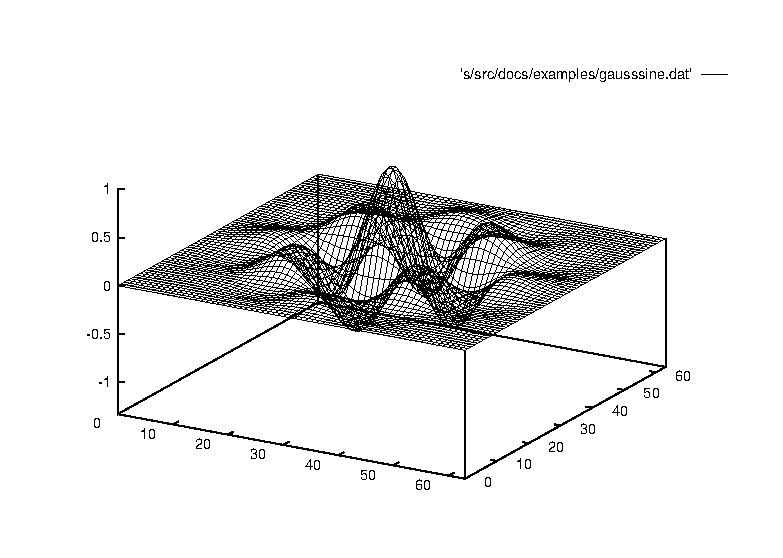
\includegraphics[width=0.75\textwidth]{sc13-gausssine-gnuplot}
\caption{File gausssine.dat, displayed with
gnuplot
}
\label{f:gausssine:g}
\end{figure}

There is good help within gnuplot, available by typing
\texttt{help}.

\subsection{IDL}
\label{s:vis-idl}

IDL is much more powerful and flexible than gnuplot, and
has a correspondingly longer learning curve.  It's never
been accused of being elegant, but with only a bit of
headbanging, I've always managed to get it to do what I
wanted (I've always seen it as reminiscent of Fortran in
this respect).

Several missions have used IDL as the language in which
they have written their data-analysis software, and
Starlink is currently experimenting with providing IDL
interfaces to important Starlink applications, which is
possible because IDL can link to codes written in
languages such as Fortran or C.  IDL is moving towards
being a core facility at Starlink sites.

IDL displays data in arrays as part of a generic set of array
manipulations.  For example, the data in the file
\texttt{gausssine.dat} was produced by the following
sequence of IDL commands:

\begin{terminalv}
x=(findgen(64)-32)^2
d=fltarr(64,64)
for i=0,63 do d(i,*)=sqrt(x+(i-32)^2)
a3=exp(-(d/15)^2)
s=sin(findgen(64)/63*5*3.141592657)
s2=s#s
m=s2*a3
\end{terminalv}

The function \texttt{findgen(N)} returns a float array
(indexed from 0 to $N-1$) in
which the value of each element is the same as its index;
performing an arithmetic operation such as subtraction or
exponentiation on an array performs it on each element of
the array; \texttt{fltarr} declares an array of floats
of the specified dimensions; the array reference
\texttt{d(i,*)} refers to the entire \texttt{i}'th
row of \texttt{d}; the operator \texttt{\#} forms
the direct product of the two vectors.  The result of this
is to set \texttt{d} to be an array where each element
is the euclidean distance from element
\texttt{(32,32)}\footnote{IDL experts will know that
the common IDL idiom for this is
\texttt{d=shift(dist(64),32,32)}, but have you ever
actually compared \texttt{dist} with its
documentation?  The documentation for \texttt{dist}
suggests that this idiom wouldn't work, but the function's
actual behaviour seems to (substantially) depart from the
claimed behaviour in exactly the right way.}.

Once we have the data in the array \texttt{m}, we can
produce a surface plot with \texttt{surface,m}, and
then go on to annotate it, rotate it, shade it, contour
it, with the large collection of options and parameters to
the \texttt{surface} command.  We can produce
PostScript output with the following sequence of commands:

\begin{terminalv}
  !p.font=0             ; use postscript fonts rather than IDL outlines
  set_plot, 'ps'        ; use the postscript output driver
  device, /encap, filename='gausssine-idl.eps'
                        ; produce encapsulated postscript
  surface, m
  device, /close        ; close the file
\end{terminalv}

This produces the EPS file shown in \ref{f:gausssine:i}.
A minor, but persistent, irritation
with IDL is that, although its input and output facilities
are as flexible as, say, Fortran's (which they closely
resemble), it doesn't come with a function for dealing
with the common case of data printed out in columns (the
only case gnuplot naturally deals with).  Fortunately,
such a function is not only easy to write, but a useful
example, too.  See \ref{a:idl}.

\begin{figure}
\center
\includegraphics[width=0.75\textwidth]{sc13-gausssine-idl}
\caption{File gausssine.dat, displayed with
IDL}
\label{f:gausssine:i}
\end{figure}

IDL comes with rather good manuals, the reference parts
of which are available on-line by typing \texttt{?} at
the IDL prompt.

See appendix B of
\xref{SUN/55}{sun55}{}
for a description of how to import data in the Starlink
NDF format into IDL.

\subsection{DX}
\label{s:dx}

IBM's Data Explorer is also available on some Starlink
machines.  I don't have personal experience of it, but
there is a Starlink manual for it in
\xref{SUN/203}{sun203}{}, ``SX and DX --- IBM data explorer
for data visualisation'' and a Starlink DX cookbook
in \xref{SC/2}{sc2}{}.

In his overview of visualisation systems in
\xref{SG/8}{sg8}{}, Clive Davenhall says of DX:

\begin{quotation}
IBM Data Explorer (DX) is a
general-purpose software package for data visualisation
and analysis. It employs a data-flow driven client-server
execution model and provides a comprehensive range of data
manipulation, visualisation and display functions.
Visualisations can be generated using a visual programming
editor or a text-based scripting language. DX is the
visualisation package recommended by Starlink,
particularly for three-dimensional scalar and vector
data. Starlink has produced a set of enhancements to
DX. If you are using DX at a Starlink site then these
enhancements should be available automatically. The use of
DX at Starlink sites and the Starlink enhancements to DX
are documented in
\xref{SUN/203}{sun203}{}.
\end{quotation}


\subsection{PGPLOT}
\label{s:pgplot}

The above recommendations describe standalone packages
which work on data produced by your code in a separate
step.  An alternative route is to incorporate the plotting
facilities within your program, and the recommended way of
doing this is by using the PGPLOT library.

The library, which was written to support astronomical
applications, consists of a collection of high-level
routines for producing plots, maps and images either
on-screen or as Postscript to a file.  Refer to
\xref{SUN/15}{sun15}{}, ``PGPLOT --- Graphics
Subroutine Library'' for further details, or to the
PGPLOT home page at \url{}.

Note that there are \emph{two} versions of PGPLOT
currently available on Starlink, `native' PGPLOT, and a
Starlink version which uses GKS.  The latter is being
deprecated, with a view to being ultimately phased out,
and this will affect how you link your program against the
library.  At the time of writing (December 1998), the way
in which the dual versions will be supported has not been
finalised; ask your system manager for advice.

\section{Producing images}
\label{s:im}

If you wish to include images in your LaTeX output, do so
using the standard graphics package.  That is, include in
your file the command \texttt{\textbackslash{}usepackage\{graphics\}} (if
you're obliged to use the old LaTeX2.09, you can use the
\texttt{epsf} option to the document style).  Include
the graphics with the command
\texttt{\textbackslash{}starincludegraphics\{file.eps\}}.  So how do you
produce the postscript?

An important point is that the postscript should be
\emph{encapsulated} postscript.  This is postscript intended to be
incorporated within another document: it has a \texttt{BoundingBox}
comment at the top of the file, and typically has the extension
\texttt{.eps}.

See \ref{s:visualisation} for details of how to produce EPS
plots from gnuplot and IDL.

If it's diagrams you want to produce, then \texttt{xfig} has its adherents.
There's a \emph{large} manual page for \texttt{xfig}, but you can do pretty
well just starting it up, and pointing and clicking.

If point and click isn't your style, try
\href{http://cm.bell-labs.com/who/hobby/MetaPost.html}{MetaPost}.
This is a variant of Knuth's MetaFont (which is used for
designing TeX fonts), which produces postscript instead.  To
produce a document using MetaPost, you produce a text file
specifying the objects you want to draw and their spatial
relationships.  It can be hard work, but the results can
look very good.  If you wished to automate producing
diagrams, perhaps because you want to produce a set of
diagrams which are systematically different, then MetaPost
could very well help you with this.  See
\texttt{.../texmf/doc/metapost} under the (Starlink) TeX
tree for further details.

\chapter{Astrophysical and other libraries}
\label{s:astro}

\section{Astrophysical modelling codes}
\label{s:models}

% <update versionid="v2-0"><px>Expanded this section
% considerably, with several more links.</px></update>
% <update versionid="v2-2"><px>Reworking of this section after
% comments from BS; added VALD and Dusty links.</px></update>

This section aims to be no more than a set of pointers to more
complete information and resources.  I'm no expert in this field,
myself, so if I've missed some important resource, or
miscontextualised something, please do let me know.

Stellar atmosphere codes:

\begin{itemize}
\item
\href{http://ccp7.dur.ac.uk/}{CCP7}
was a
\href{http://www.dci.clrc.ac.uk/ListActivities.asp?Class=5;Classtype=21;}{Collaborative Computational Project},
`concerned with the
calculation of theoretical models suitable for the
interpretation of stellar and interstellar spectra'.
As well as promoting the use of advanced computers in
astronomy, it developed a library of
stellar-atmosphere and spectroscopy codes.  The
project finished in April 2001, but the resources it
produced are still useful.

\item
\href{http://star.arm.ac.uk/~csj/}{Simon Jeffery}
makes available a number of tools
for stellar atmosphere calculations.

\item
At \href{http://kurucz.harvard.edu/}{Robert Kurucz's home page}
you can obtain copies of
his ATLAS and other codes, along with grids of model
atmospheres.

\item
\href{http://phoenix.physast.uga.edu/}{PHOENIX}:
state-of-the-art M-star model atmospheres.
\end{itemize}

Atomic and molecular data:

\begin{itemize}
\item
The \href{http://vizier.u-strasbg.fr/OP.html}{Opacity Project}
is a collaborative project to
produce the atomic data required for stellar
envelope calculations.  The project makes the
results generally available both through a database
called `TOPbase', and by anonymous FTP.

\item
Other opacity data is available from the
\href{http://www-phys.llnl.gov/V_Div/OPAL/}{OPAL code}.
As well as making precalculated
opacity tables available, you can make requests for
new tables to be generated.

\item
Atomic data at \href{http://www.pa.uky.edu/~verner/atom.html}{Kentucky}
and \href{http://cfa-www.harvard.edu/amdata/ampdata/amdata.html}{Harvard}

\item
\href{http://spec.jpl.nasa.gov/}{JPL Molecular Spectroscopy}

\item
The \href{http://www.astro.univie.ac.at/~vald/}{Vienna Atomic Line Database (VALD)}
is an excellent
site with up-to-date atomic data needed for spectrum
synthesis.
\end{itemize}

Astronomical chemistry (loosely) --- dust, clouds and the
interstellar medium:

\begin{itemize}
\item
\href{http://www.pa.uky.edu/~gary/cloudy/}{Cloudy}
is a arge-scale plasma simulation code that is widely
used across the astronomical community as an aid in
the interpretation of spectroscopic data.

\item
\href{http://www.pa.uky.edu/~moshe/dusty/}{DUSTY}
is a dust-shell modelling code, also originating at
Kentucky.
\end{itemize}

A number of
\href{http://www.fges.demon.co.uk/cfd/CFD\_codes.html}{CFD codes}
are available to buy or download.  This is a
collection of pointers and notes about a large number of CFD
codes, from a variety of sources.

Thanks to [\hyperlink{ta:sj}{SJ}], [\hyperlink{ta:bs}{BS}] and
[\hyperlink{ta:as}{AS}] for
much of the content of this section.


\section{General-purpose and numerical libraries}
\label{s:lib}

% <update versionid="v2-0"><px>Longer discussion of the GPL
% and other free licences.</px></update></subhead>

There are numerous software libraries available.  Many of
these are free, many are public domain.  The difference
between the two is that `public-domain software' is in some
sense `ownerless': it's yours to play with, or modify, or
exploit, as you wish, with only good manners requiring you
to acknowledge the source (this is not an authoritative
statement of copyright law, by the way...).  `Free'
software, on the other hand, is still copyrighted, but you
may have a free licence to use it for certain purposes.  One
of the best known of these licences is the
\href{http://www.gnu.org/copyleft/gpl.html}{GNU General Public Licence},
which gives you very good access to
the code, limited only by the requirement that programs
produced using GPL'd code are themselves made as freely
availale.  Other licences might make the code available to
academic users only, or only for non-commercial use.  The
GNU project have a useful collection of
\href{http://www.gnu.org/licenses/license-list.html}{free and not-so-free licences},
which is useful even though
they are sometimes a little fervent about the issues.  The
type of licence makes a difference if you plan to
redistribute your code.  See also the observations about
libraries, and thoughtless use of them, in \ref{s:na}.

Probably the most commonly used numerical library is the
\href{http://www.nag.co.uk}{NAG library}.
This is a long-established, and very highly thought-of,
library, which contains codes to deal with a broad range of
numerical problems.  The routines tend to come in several
versions, typically a highly general, and highly
configurable, one, accompanied by easy-to-use drivers.  The
NAG library is expensive, but Starlink's size allows it to
negotiate with NAG to provide the library at all Starlink
sites.  The routines are generally in Fortran, but C
versions of some of them are becoming available.

The PDA library is a collection of public-domain and free routines,
assembled by Starlink, and intended to replace the NAG library in
Starlink application code.  The collection was assembled using GAMS,
with routines drawn from FFTPACK, SLATEC,
NMS, OPT, plus other isolated sources.  If you need
to use one of the available algorithms, then the
advantage of using the library version is that the (possibly
non-trivial) work of building it for your architecture has already
been done, leaving you able to simply link against the library.  The
collection is fully documented in
\xref{SUN/194}{sun194}{}.

The remaining libraries are typically free.

In your search for codes, you would do well to start at
\href{http://gams.nist.gov}{GAMS}: Guide to
Available Mathematical Software.  This describes itself as
`A cross-index and virtual repository of mathematical and
statistical software components of use in computational
science and engineering'.  You can either search for the
code you need by keyword, or work through their
classification of problems (a classification which is
occasionally used more widely) to find references.  They
point to both free and commercial software.

The first collection to be aware of is Netlib.  The archive
is based at \url{http://www.netlib.org}, but there are
\href{http://www.netlib.org/bib/mirrors.html}{UK mirrors}
Although there are some facilities which
are primarily available at Netlib, it also mirrors several
other archives.

\href{http://www.nhse.org/}{NHSE}, the (US) National
High-Performance Software Exchange, is `a distributed
collection of software, documents, data, and information of interest
to the high performance and parallel computing community'.
NHSE is part of Netlib, and incorporates software repositories
\href{http://www.nhse.org/hpc-netlib/}{HPC-netlib}
for
high-performance software,
\href{http://www.nhse.org/ptlib/}{PTlib}
for parallel tools,
and \href{http://www.csir.org/}{CSIR}
for chemistry software.

The
\href{http://wwwinfo.cern.ch/asd/index.html}{CERN program library}
includes \href{http://wwwinfo.cern.ch/asd/cernlib/overview.html}{CERNLIB},
which consists of a number of
\href{http://wwwinfo.cern.ch/asd/cernlib/libraries.html}{component libraries}.
This is a long-standing and well-known
library of general-purpose Fortran (typically) numerical
routines with, obviously, some bias towards particle
physics.  The service is free to all HEP users, and to
physics departments in CERN member states, with separate
non-commercial and commercial rates available.  There is a
\href{http://wwwinfo.cern.ch/asdcgi/listcernlibfaqs.pl}{FAQ}.

JPL has a
\href{http://math.jpl.nasa.gov/}{Computational Mathematics Library}.
These appear to be free, but no longer
formally supported by JPL.

The
\href{http://math.nist.gov/toms/Overview.html}{ACM Transactions on Mathematical Software}
(TOMS) is a
journal produced by the ACM.  The software discussed in
there is available at GAMS, and mirrored at
\href{http://www.hensa.ac.uk/netlib/toms/}{HENSA}.

The
\href{http://www.scd.ucar.edu/}{Scientific Computing Division}
of the (US)
\href{http://www.ncar.ucar.edu/}{National Center for Atmospheric Research},
has an overview of
\href{http://www.scd.ucar.edu/softlib/mathlib.html}{mathematical and statistical packages}.
Not all the packages
reviewed there are freely available, but the discussions are
useful.

\href{http://www.bell-labs.com/project/PORT/}{PORT}
is a collection of general maths subroutines.  Its description of
itself is on the front page: `The
PORT Mathematical Subroutine Library (third edition) is a
collection of Fortran 77 routines that address many
traditional areas of mathematical software, including
approximation, ordinary and partial differential equations,
linear algebra and eigensystems, optimization, quadrature,
root finding, special functions, and Fourier transforms, but
excluding statistical calculations. PORT stands for Portable,
Outstanding, Reliable, and Tested.'
Some routines are public-domain when, for example, they are
developments of public routines, others have a
non-commercial-use licence condition.

\href{http://www.hensa.ac.uk/netlib/slatec/index.html}{Slatec}
is `a comprehensive software library containing over 1400
general purpose mathematical and statistical routines
written in Fortran 77.'

Specifically concerned with minimisation,
\href{http://www.hensa.ac.uk/netlib/minpack/}{minpack}
(or at \href{http://www.netlib.org/minpack/}{netlib}), is a
library for solving linear and nonlinear minimisation
problems.  It has documentation within the source code.

\subsection{Reading and writing data}
\label{s:rwdata}

% <update versionid="v2-0"><px>Added CONVERT example, and
% added pointers to FITS and cfitsio.</px></update>

The codes you write do not exist in isolation, and at
some point you will have to read data from, or write it
to, files.  You might, therefore, need to read or write
one of a number of standard data formats.  Clive Davenhall
wrote an article on this in the September 1998 issue of the
\href{http://www.starlink.ac.uk/bulletin/98sep/node12.html}{Starlink Bulletin}.
This covered reading and writing using
the IMG library (\xref{SUN/160}{sun160}{}),
using NDF files and the HDS files they are a special case
of (\xref{SUN/33}{sun33}{} and \xref{SUN/92}{sun92}{} respectively),
and reading and writing FITS files
(\xref{SUN/136}{sun136}{}).

You can convert between different data formats using the
CONVERT package, documented in \xref{SUN/55}{sun55}{}.
CONVERT is extremely easy to use, and
converting a FITS file, say, to an NDF is as easy as

\begin{terminalv}
fits2ndf myfile.fits myfile
\end{terminalv}

If you have to read or write FITS files, then visit the
\href{http://fits.gsfc.nasa.gov/}{FITS home page}
for the FITS users guide and the
\href{http://heasarc.gsfc.nasa.gov/docs/software/fitsio/fitsio.html}{\texttt{cfitsio}}
library.  Although FITS files have a very simple format,
there are enough ways of getting things wrong that you
will, as usual, save yourself time in the long run by
taking the trouble to use the \texttt{cfitsio}
library.  It's easier than you might think: the Quick
Start Guide contains most of what you'll ever need to
know.  Note that, although the library is called
\emph{c}fitsio, it's designed to be used with Fortran as
well, and the programmer's reference guide comes in two
flavours.

Once the data is there, you will need to visualise it.  See
\ref{s:im} for some pointers to suitable
software.

\section{Link farms}
\label{s:link:libs}

\url{http://cdsweb.u-strasbg.fr/astroweb.html}:
AstroWeb is one of the most useful link collection, because
it has been developed by the astronomy community.

\url{http://math.nist.gov/toms/Resources.html}: The
TOMS list of web resources for mathematical software is a
collection of pointers maths software on the web.

Yahoo has managed to assemble a respectable collection of
pointers to Scientific software at
\url{http://uk.yahoo.com/Computers_and_Internet/Software/Scientific/},
as well as more specific pointers to maths
(\url{http://uk.yahoo.com/Science/Mathematics/Software/}),
physics
(\url{http://uk.yahoo.com/Science/Physics/Software/})
and astronomy
(\url{http://uk.yahoo.com/Computers_and_Internet/Software/Scientific/Astronomy/})
resources.

\chapter{Paper production}
\label{s:paper}

\section{TeX and LaTeX}
\label{s:latex}

% <update versionid="v2-0"><px>Pointers to the LaTeX project, other tutorials, and the TeX FAQ.
% Some reorganisation.</px></update>
% <update versionid="v2-3"><px>Added a
% reference to the Adam Lewenberg book
% pointers</px></update>
% <update versionid="v2-5"><px>Added
% a pointer to Peter Flynn's Beginner's
% LaTeX</px></update>

Starlink supports LaTeX and TeX users by maintaining and
packaging for release a TeX distribution.  This is typically based
on one of the standard TeX distributions, plus an effort to ensure
that the distribution includes packages of interest to astronomers,
particularly some of the relevant journal style files.  See the
\href{http://www.starlink.ac.uk/%7eacc/tex/tex.html}{Starlink LaTeX page}
for details.

\href{http://www.latex-project.org/}{LaTeX} is
nominally (though not actually)
re-released every six months, in June and December, with
each release incorporating bugfixes, but no significant development.
New features are being incorporated into LaTeX3, which is a major
upgrade, still being developed.  Versions more than a year old (that
is, more than two releases ago) are formally `obsolete', and bug reports
won't be accepted for them.

The current version of LaTeX is also known as LaTeX2e, to
distinguish it from the by now completely obsolete LaTeX2.09, which
is the version of LaTeX described in the first edition of Lamport's
book.  LaTeX2e has significant internal differences from
LaTeX2.09, but was intended to appear much the same to the user.
The most prominent difference is that LaTeX2e files start with the
declaration \texttt{\textbackslash{}documentclass[options]\{classname\}}, and
invoke further packages using \texttt{\textbackslash{}usepackage\{packagename\}},
whilst LaTeX2.09 files start
\texttt{\textbackslash{}documentstyle[options]\{stylename\}}, with the options list
being a mixture of style file options and package names.  LaTeX2e
will attempt to go into a `compatibility mode' if it sees a file start
with \texttt{\textbackslash{}documentstyle}, but this isn't terribly reliable,
and you \emph{certainly} shouldn't create new files like this,
unless some primitive publisher (which used to include MNRAS until
rather recently) absolutely insists on it.

Other LaTeX resources you might want to examine are the
\href{http://www.tex.ac.uk/faq}{UK TeX FAQ} (this is \emph{very} good),
\href{http://wwwinfo.cern.ch/asdoc/textproc.html}{CERN's TeXpages},
and the \href{http://www.tex.ac.uk/tex-archive/help/Catalogue/catalogue.html}{catalogue}
at \href{http://www.tex.ac.uk}{CTAN}
(the `Comprehensive TeX Archive Network', hosted on three peer
machines in the UK, Germany and the US, and mirrored
worldwide; all TeX is there).

All this, of course, assumes that you're already a LaTeX user.
If you're just starting with LaTeX, then the canonical place to
start is with Leslie Lamport's
``LaTeX: a Document Preparation System, 2nd edition'' \citep{lamport}.
I think this is a good
introduction, because it concentrates on the basics, and leaves the
elaborate details to others.  The bulk of the book is an accessible
introduction to LaTeX (and note that you really ought to avoid asking
LaTeX questions until you've read chapter 2); appendix C is
a reference manual.

If it's the elaborate details you
want, then you'll need to supplement Lamport.  Victor Eijkhout's
\href{http://www.eijkhout.net/tbt/}{TeX by Topic} is
well spoken-of, though I haven't examined it myself (the book is now out
of print, but the author has made it available for free, for a donation).
Two other good books to
examine are
``A Guide to LaTeX'' \citep{kopka},
and ``LaTeX Line by Line'' \citep{diller}.
Both are substantially more advanced than Lamport,
and cover a lot of material densely but reasonably clearly.  If forced
to choose, I would go for Kopka and Daly over Diller, partly because
they have produced a second edition covering LaTeX2e, but also
because Diller seems to try to pack in too much, including some
material (such as the intricacies of maths typesetting) which, if
you're going to learn, you should probably learn from Knuth's TeXbook.
Having said that, the advantage is a narrow one, and you'd be
well-advised to choose based on whose writing style you prefer, and
which one happens to be in the bookshop on the right day\footnote{It's
unfortunate that neither book is much of an advert for TeX's
potentially beautiful typesetting --- both seem to be produced using a
practically unmodified LaTeX \texttt{book} style.}.
Both of the last two should be kept away from anyone not already convinced of
LaTeX's virtues, since they both make LaTeX seem much
more forbidding than it actually is.
Finally, Goossens,
Mittelback and Samarin's
``The LaTeX Companion'' \citep{goossens}
is useful, but intended as a reference, not as an
introduction.  For other print books, and details of these ones, see the
TeX FAQ's bibliography at
\url{http://www.tex.ac.uk/cgi-bin/texfaq2html?label=books}, and Adam
Lewenberg's collection of
\href{http://www.macrotex.net/texbooks/}{TeX and LaTeX print resources}.

There are a number of
\href{http://www.tex.ac.uk/cgi-bin/texfaq2html?label=tutorials}{online tutorials}.
Both the `\href{http://www.tex.ac.uk/tex-archive/info/gentle/}{Gentle Introduction}'
and the `\href{http://www.tex.ac.uk/tex-archive/info/lshort/english/}{Not so Short Introduction}'
are available at CTAN.  Peter Flynn's
`\href{http://www.silmaril.ie/downloads/documents/beginlatex.pdf}{Beginner's LaTeX}'
is well written and informative, and
spends a good deal more time on the preliminary technicalities than
others; but --- since it grew out of a two-day introduction to LaTeX
aimed primarily at humanities users --- it does not cover maths.

% XXX: possibly include pointers to
% http://www-h.eng.cam.ac.uk/help/tpl/textprocessing/
% http://www.latex-project.org/

If you prefer learning by example, take a look at the standard sample
files, \texttt{small2e.tex} and \texttt{sample2e.tex}.  These will be
somewhere in your LaTeX distribution, typically with a path ending
in \texttt{.../tex/latex/base/small2e.tex} (try \texttt{echo \$TEXINPUTS}
or \texttt{kpsepath tex} to help locate the TeX
distribution on your local machine).

\emph{The} book on TeX is Knuth's original,
``The TeXbook'' \citep{knuth}.  As well as describing
the underlying TeX engine, this also
describes Knuth's very basic macro package, \texttt{plain}.  You need
the TeXbook if you're writing a LaTeX macro package, if you
demand complete control over positioning (tricky in TeX, but an
out-and-out hassle in LaTeX), or if you just don't like the way
LaTeX lays things out and want to do it all yourself.  If you don't
fall into any of those categories, \texttt{plain} TeX is probably
not where to start (and I speak as a lapsed TeXie who has spluttered
furiously at Leslie Lamport's failure to impose a satisfactorily
rigourous line on even such fundamental doctrinal matters as how the
word `LaTeX' is to be pronounced).

You should be aware of \texttt{pdflatex}, which is a version of
TeX which produces PDF files directly rather than DVI files (though
note that versions before \texttt{1.0-prerelease} produce bad PDF
which breaks Windows Acroread 5 at least).

Starlink has produced several documents concerned with LaTeX.
The LaTeX user's guide,
\xref{SUN/9}{sun9}{},
concentrates on the practical details of LaTeXing your document and
ultimately transforming it into PostScript.  You should also refer to
\xref{SC/9}{sc9}{}, the LaTeX cookbook.
However, \xref{SGP/28}{sgp28}{}, ``How to write good
documents for
Starlink'', \xref{SUN/199}{sun199}{}, \emph{Star2HTML} and
\xref{SGP/50}{sgp50}{}, ``Starlink Document Styles'' are
primarily intended for those writing Starlink
documentation.

\section{The LANL archive}
\label{s:lanl}

The LANL preprint archive is based, in the UK, at
\url{http://xxx.soton.ac.uk} which is a mirror of the
\href{http://xxx.lanl.gov}{master archive} at
LANL.  The archive is easy to use as a reader but not,
unfortunately, transparently easy to use as an author (not
helped by the rather snide error messages that come back if
you slip up...).

The \href{http://xxx.soton.ac.uk/help/}{full instructions}
are comprehensive, but boil down to
the following:

\begin{itemize}
\item
The first time you submit
anything to the archive, you need to register as an
author.  That registers your email address with them and
sets a few preferences (such as the default archive you'll
submit to).

\item
Bundle up the LaTeX source for
your paper in a \texttt{.tar.gz} archive.  The
automatic-processing software at LANL seems to LaTeX every
\texttt{.tex} file in sight, so if your submission
isn't in the canonical format of one TeX file plus a bunch
of PostScript figures, you'd probably best read the
instructions one more time.  It follows from this that it
doesn't matter what you call your TeX file: the processing
software will still TeX it.

LANL has copies of
journal styles such as the A\&A one --- when they
process your paper it'll be formatted according to that
style file.  They suggest that the PostScript figures in
the article be numbered something like
\texttt{figure1.ps}, \texttt{figure2.ps}, so that
they alphabetise correctly.  See
\href{http://xxx.soton.ac.uk/help/submit_tex}{``Considerations for TeX submissions''}
for the gory details.

\item
Read the uploads help again,
particularly the information on the information fields
you'll have to fill in, then go to the uploads page at
\url{http://xxx.lanl.gov/uploads}.

\item
The uploads page gives you a form to type in the various
details of author and title and the like, and to type in
the abstract.  You give the name of your tar file, press
the button and wait.  After a pause you can check if the
automatic processing succeeded.  At this stage, you'll be
given a password for this paper.  This allows you and your
co-authors to retrieve the paper before it's put in the
public archive, and will be needed to make alterations, or
update the journal publication details, in
future.

\item
Now, you need a drink.
\end{itemize}

\chapter{General astronomical and astrophysical resources}
\label{s:astro:general}

The \href{http://cdsads.u-strasbg.fr/}{Astrophysics Data System} (ADS)
is a NASA project, providing an
abstract service, along with a subsidiary data service.
Further to this, \xref{SUN/174}{sun174}{},
``An Astronomer's Guide to On-line Bibliographic Databases
and Information Services'', describes bibliographic and
other resources of interest to astronomers.

\section{Observations}
\label{s:obs}

\href{http://simbad.u-strasbg.fr/Simbad}{SIMBAD} is a
`Set of Identifications, Measurements and Bibliography for
Astronomical Data'.  It's a large database (5,416,970
objects in November 1998) of astronomical objects, which you
can search by identifier, coordinates, or other sampling
criteria.  As well as basic data for the objects, it
includes some observational data from, and journal
references to, the object.  You have to register before you
can use it; it's not free, but if you're in the US or in an
ESO or ESA member state, the costs are covered for you.
Also at CDS is the 
\href{http://cdsweb.u-strasbg.fr/Cats.html}{CDS catalogue service},
which allows you to search a list of
almost 3000 catalogues, plus the contents of tables
published in A\&A.

If you're using such catalogues, you might want to take a
look at CAT, the Starlink ``Catalogue and table
manipulation library'', documented in
\xref{SUN/181}{sun181}{}.  This is a subroutine
library for manipulating astronomical catalogues and similar
tabular datasets.  See also
\xref{SUN/127}{sun127}{}, ``The EXOSAT Database System'',
and more generally \xref{SUN/162}{sun162}{},
``A Guide to Astronomical Catalogues, Databases and
Archives available through Starlink''.

\chapter{Acknowledgements}
\label{s:acknowledgements}

A number of people have contributed to this document, either
with helpful general remarks or corrections or amplifications on
points of detail.  Where their contribution was precisely localisable
--- in particular where I have merely sub-edited their comments into
place --- they are also acknowledged at the appropriate specific points
in the text.

\begin{itemize}
\item
\hypertarget{ta:sg}{SG}: Sergio Gelato
(\texttt{Sergio.Gelato@Durham.ac.uk}) added remarks
about optimizing C, and compiler switches.

\item
\hypertarget{ta:sj}{SJ}: Simon Jeffery
(\texttt{csj@star.arm.ac.uk}) added pointers to model
atmosphere codes.

\item
\hypertarget{ta:jl}{JL}: Jon Lockley
(\texttt{jjl@astro.soton.ac.uk})

\item
\hypertarget{ta:as}{AS}: Anne Sansom
(\texttt{aesansom@uclan.ac.uk}).

\item
\hypertarget{ta:bs}{BS}: Barry Smalley
(\texttt{bs@astro.keele.ac.uk}). Pointers to model
atmospheres.

\item
\hypertarget{ta:mbt}{MBT}: Mark Taylor
(\texttt{mbt@ast.cam.ac.uk}) made a number of points
about my coverage of Fortran, and several insightful
remarks about numerical programming.

\item
\hypertarget{ta:rfws}{RFWS}: Rodney Warren-Smith made many
comments on an early draft of the text, which made it
much better than it otherwise might have been.

\item
\hypertarget{ta:rw}{RW}: Robin Williams
(\texttt{Robin.Williams@astro.cf.ac.uk}) general
comments, and information about Alpha switches.
\end{itemize}

\appendix

\chapter{Example programs}
\label{s:examples}

% <update versionid="v2-0"><px>Added islittleendian example
% program</px></update>
% <update versionid="v2-1"><px>Added download
% URL</px></update>

This section contains several example programs.  These are also
distributed with the source of this document.  Look in \texttt{/star/examples/sc13*}.  The examples are available
for download from
\url{http://www.astro.gla.ac.uk/users/norman/star/sc13/sc13-examples.tar.gz}.

\section{islittlendian.c}
\label{a:islittleendian:c}

If you want to find out, possibly as part of a script,
whether a particular platform is big- or little-endian,
the information will probably be squirrelled away
somewhere in the headers for the compiler you're using,
unfortunately not in any standard way.  However, a
portable way of doing this (which incidentally illustrates
the contrast between the two systems) is to use this
little program.  It isn't bullet-proof, but if it fails,
this is probably the least of your cross-platform
problems.  You can use the program as follows:

\begin{terminalv}
% echo '#define BIGENDIAN' \
    `if ./islittleendian; then echo 0; else echo 1; fi` >bytesex.h
\end{terminalv}

to create a file \texttt{bytesex.h} with either \texttt{\#define BIGENDIAN 1}
or \texttt{\#define BIGENDIAN 0} in it.

\verbatiminput{examples/islittleendian.c}

\section{fpp.c}
\label{a:fpp:c}

% <update versionid="v2-0"><px>Replaced with expanded/corrected program, which also deals with
% doubles.</px></update>

The first \texttt{fpp.c}, allows you to explore the representation of
floating-point numbers on your machine.  Note that machines may have
either `big-endian' or `little-endian' addressing schemes (referring
to the order in which integers and floating-point numbers are stored
in memory).  Alpha and Intel chips are little-endian, Sparcs, the
Motorola 68k family used in Macs, and Motorola PowerPC chips, are
big-endian.  On the latter machines, you'll need to compile these
programs with the \texttt{-DBIGENDIAN} option to the C compiler.

\verbatiminput{examples/fpp.c}

\section{fpdemo.c}
\label{a:fpdemo:c}

The program \texttt{fpdemo.c} is discussed in
section \ref{s:accuracy}, and shows the effects of catastrophic
cancellation.

\verbatiminput{examples/fpdemo.c}

\section{Profiling}
\label{a:profiling}

The fortran files \texttt{p?.f} are example files for
\ref{s:profiling}, on profiling.  These are drawn
from \citet{sunf77}.

\subsection{p1.f}

\verbatiminput{examples/p1.f}

\subsection{p2.f}

\verbatiminput{examples/p2.f}

\subsection{p3.f}

\verbatiminput{examples/p3.f}

\section{crash.c}
\label{a:crash:c}

The program \texttt{crash.c} crashes and dumps core.
See \ref{s:debugging} for discussion.

\verbatiminput{examples/crash.c}

\section{Mixed language programming}
\label{a:mixed}

The files \texttt{mixed-c.c} and \texttt{mixed-f.f}
illustrate some of
the techniques involved in calling C from Fortran and
\emph{vice versa}, as described in \ref{s:candf}.

On a Sun, compile and link them as follows:

\begin{terminalv}
f77 -c mixed-f.f -ext_names=plain
cc -c mixed-c.c
f77 -o mixed mixed-c.o mixed-f.o
\end{terminalv}

The extra option to the first \texttt{f77} command
tells the compiler not to add an underscore to function
names; different compilers will have different switches
for accomplishing the same thing.  See \ref{s:compilingcf} for discussion.

\subsection{mixed-c.c}

\verbatiminput{examples/mixed-c.c}

\subsection{mixed-f.f}

\verbatiminput{examples/mixed-f.f}

\section{maple.ms}
\label{a:maple}

This example Maple file gives a slightly fuller example
of Maple use than given in \ref{s:maple}.

\verbatiminput{examples/maple.ms}

\section{idl-functions.pro}
\label{a:idl}

Here is an example of IDL programming, dealing with the common
situation of reading in columns of data.  See also
\ref{s:vis-idl}.

\verbatiminput{examples/idl-functions.pro}

\chapter{References: Starlink documents}
\label{s:refs}

This section contains a (non-exhaustive!) selection of Starlink
documents which should intersect with the interests of this cookbook's
audience.  Where possible, I have included a reference to a relevant
section of this document.

An overall reference for all Starlink users is the
\xref{Starlink User's Guide}{sug}{}.

\begin{tabular}{lp{4in}r}
\multicolumn{3}{c}{Starlink User Notes}                                                                     \\
Code                     & Title                                                    & Sect.                 \\
\xref{SUN/1}{sun1}{}     & Starlink software collection                             &                       \\
\xref{SUN/9}{sun9}{}     & LaTeX --- Document preparation system v2e User's Guide   & \ref{s:latex}         \\
\xref{SUN/11}{sun11}{}   & ARY --- Subroutines for accessing ARRAY data structures  &                       \\
\xref{SUN/12}{sun12}{}   & LaTeX --- Cook-book                                      & \ref{s:latex}         \\
\xref{SUN/15}{sun15}{}   & PGPLOT --- Graphics subroutine library                   & \ref{s:pgplot}        \\
\xref{SUN/28}{sun28}{}   & NAG --- Numerical and Graphical Libraries Mk 16/4 UG     & \ref{s:lib}           \\
\xref{SUN/33}{sun33}{}   & NDF --- Routines for accessing extensible n-D data 1.3   & \ref{s:rwdata}        \\
\xref{SUN/55}{sun55}{}   & CONVERT --- A format-conversion package 1.1, UM          & \ref{s:vis-idl}       \\
\xref{SUN/73}{sun73}{}   & FORCHECK --- Fortran verifier and programming aid        & \ref{s:fortran77}     \\
\xref{SUN/92}{sun92}{}   & HDS --- Hierarchical data system 4.2, PG                 & \ref{s:rwdata}        \\
\xref{SUN/93}{sun93}{}   & TeX --- Superior document preparation system             & \ref{s:latex}         \\
\xref{SUN/107}{sun107}{} & MAPLE --- Mathematical manipulation language             & \ref{s:maple}         \\
\xref{SUN/127}{sun127}{} & EXOSAT database system                                   & \ref{s:obs}           \\
\xref{SUN/136}{sun136}{} & FITSIO --- Disk FITS I/O routines 5.03                   & \ref{s:rwdata}        \\
\xref{SUN/145}{sun145}{} & UNIX --- An introduction                                 & \ref{s:unix}          \\
\xref{SUN/160}{sun160}{} & IMG --- Simple image data access 1.2                     & \ref{s:rwdata}        \\
\xref{SUN/162}{sun162}{} & A guide to astronomical catalogues/databases/archives    & \ref{s:obs}           \\
\xref{SUN/167}{sun167}{} & PERIOD --- A time-series analysis package                &                       \\
\xref{SUN/170}{sun170}{} & Editors on Unix                                          & \ref{s:unix}          \\
\xref{SUN/172}{sun172}{} & FTNCHEK --- A Fortran 77 source-code checker             & \ref{s:fortran77}     \\
\xref{SUN/174}{sun174}{} & Guide to on-line bibliographies and information          &                       \\
\xref{SUN/181}{sun181}{} & CAT --- Catalogue and table manipulation library 5.1     & \ref{s:obs}           \\
\xref{SUN/193}{sun193}{} & PERL --- Practical Extraction and Report Language        & \ref{s:otherlang}     \\
\xref{SUN/194}{sun194}{} & PDA --- Public domain algorithms library 0.4, PM         & \ref{s:lib}           \\
\xref{SUN/203}{sun203}{} & SX and DX --- IBM data explorer for data visualisation   & \ref{s:dx}            \\
\xref{SUN/209}{sun209}{} & CNF and F77 Mixed Language Programming v3.1: PM.         & \ref{s:candf}         \\
\end{tabular}

\begin{tabular}{lp{4in}r}
\multicolumn{3}{c}{Starlink General Papers}                                                                 \\
\xref{SGP/4}{sgp4}{}     & Starlink C programming standard                          & \ref{s:c}             \\
\xref{SGP/16}{sgp16}{}   & Starlink application programming standard                & \ref{s:fortran77}     \\
\xref{SGP/47}{sgp47}{}   & Computer Algebra Software                                & \ref{s:maple}         \\
\end{tabular}

\begin{tabular}{lp{4in}r}
\multicolumn{3}{c}{Starlink Cookbooks}                                                                      \\
\xref{SC/2}{sc2}{}       & The DX cookbook                                          & \ref{s:dx}            \\
\xref{SC/9}{sc9}{}       & LaTeX Cookbook                                           & \ref{s:latex}         \\
\xref{SC/12}{sc12}{}     & Writing your own data reduction software                 &                       \\
\end{tabular}

\begin{tabular}{lp{4in}r}
\multicolumn{3}{c}{Starlink Guides}                                                                         \\
\xref{SG/6}{sg6}{}       & ADAM --- Programmer's facilities and documentation guide &                       \\
\xref{SG/8}{sg8}{}       & Introduction to Visualisation Software for Astronomy     & \ref{s:visualisation} \\
\end{tabular}

Miscellaneous User Documents are documents which are not
originated by Starlink, which are held at RAL for the
Starlink project. Copies may be available at other Starlink
nodes. Ask your Site Manager if you want one.

\begin{tabular}{lp{4in}r}
\multicolumn{3}{c}{Miscellaneous User Documents}                                                            \\
\xref{MUD/30}{mud30}{}   & IDL --- User's guide                                     & \ref{s:vis-idl}       \\
\xref{MUD/48}{mud48}{}   & LATEX --- User's guide and reference manual              & \ref{s:latex}         \\
\xref{MUD/52}{mud52}{}   & MAPLE --- Introduction                                   & \ref{s:maple}         \\
\xref{MUD/55}{mud55}{}   & NAG --- Fortran library manual: Mk 15 (10 vols)          & \ref{s:lib}           \\
\xref{MUD/56}{mud56}{}   & NAG --- A beginners guide (Book)                         & \ref{s:lib}           \\
\xref{MUD/57}{mud57}{}   & NAG --- Newsletters, Error bulletins                     & \ref{s:lib}           \\
\xref{MUD/58}{mud58}{}   & NAG --- Graphical library supplement: Mk 3 (2 vols       & \ref{s:lib}           \\
\xref{MUD/72}{mud72}{}   & TEX --- The TeXbook (Book)                               & \ref{s:latex}         \\
\xref{MUD/121}{mud121}{} & Unix for beginners                                       & \ref{s:unix}          \\
\xref{MUD/122}{mud122}{} & An introduction to display editing with Vi               & \ref{s:editors}       \\
\xref{MUD/123}{mud123}{} & Vi --- Quick reference card                              & \ref{s:editors}       \\
\xref{MUD/128}{mud128}{} & NAG --- Fortran Library, Introductory Guide (Mk 15)      & \ref{s:lib}           \\
\xref{MUD/137}{mud137}{} & MAPLE V --- Language reference manual                    & \ref{s:maple}         \\
\xref{MUD/138}{mud138}{} & MAPLE V --- Library reference manual                     & \ref{s:maple}         \\
\xref{MUD/139}{mud139}{} & MAPLE V --- A tutorial introduction                      & \ref{s:maple}         \\
\xref{MUD/159}{mud159}{} & SM --- Interactive plotting program 2.3.1                & \ref{s:visualisation} \\
\xref{MUD/160}{mud160}{} & SM --- The SM tutorial                                   & \ref{s:visualisation} \\
\end{tabular}

\chapter{Release notes}
\label{s:relnotes}

\section{Release 2.5 (10-Mar-2003)}

Minor edits, plus repackaging

\section{Release 2.4 (22-Jul-2002)}

Minor edits for clarity, and to restore missing
references.

\section{Release 2.3 (16-Jul-2002)}

Minor edits --- typos and enhancements spotted now and
again.

\section{Release 2.2 (01-Dec-2001)}
\label{rel-2.2}

\begin{itemize}
\item
Enhanced the coverage of Java (though it's still rather brief).

\item
Added pointers to stellar atmosphere codes (thanks to Barry
Smalley, Ann Sansom, Simon Jeffery).

\item
A few additions to the TeX/LaTeX coverage.
\end{itemize}

\section{Release 2.1 (04-Dec-2001)}
\label{rel-2.1}

More detail about NaNs, compilers, largely incorporating the suggestions
I received after the previous edition.  Packaged set of examples.

\section{Version 2 (02-Dec-2001)}
\label{rel-2.0}

Assorted enhancements and additions.  Expanded the section on model
atmospheres.  Links checked, and a couple of broken ones restored.

I haven't been able to incorporate all the suggestions I received
after the previous edition.

\section{Release 1.2}
\label{rel-1.2}

No significant changes as yet.  Merely a conversion from the
original LaTeX source.

\section{Release 1.1 (20-Jun-2000)}

Incorporating comments from others.

\chapter{Bibliography}

\bibliography{sc13}
\bibliographystyle{plainnat}

\end{document}
